\documentclass[11pt,a4paper]{article}
\usepackage[utf8]{inputenc}
\usepackage[T1]{fontenc}
\usepackage{amsmath,amsfonts,amssymb}

\usepackage{apacite}
\usepackage{natbib}
\usepackage{graphicx}
\usepackage{booktabs}
\usepackage{threeparttable}
\usepackage{array}
\usepackage{url}
\usepackage{hyperref}
\usepackage[margin=2.5cm]{geometry}
\usepackage{setspace}
\usepackage{comment}
\usepackage{outlines}
\onehalfspacing
%\doublespacing

\newcommand{\tablepath}{papers/econometrics/table}
\newcommand{\figurepath}{papers/econometrics/figure}

\newcommand{\Var}{\text{Var}}
\newcommand{\Cov}{\text{Cov}}

\DeclareMathOperator*{\plim}{plim}

% Define \sym command for significance stars from esttab
\newcommand{\sym}[1]{{#1}}

\title{CEO Replacements and Firm Growth: Correcting for Small-Sample Bias in Fixed-Effect Estimates\thanks{We thank Ot\'{a}vio Bartalotti and St\'ephane Bonhomme for helpful discussions and comments.  We thank the excellent assistance provided by Gergely Attila Kiss. The paper benefited from presentations at the Universit\'a della Svizzera Italiana and Corvinus Empirical Seminar. Project No. 144193 has been implemented with the support provided by the Ministry of Culture and Innovation of Hungary from the National Research, Development and Innovation Fund, financed under the KKP\_22 funding scheme. This project was funded by the European Research Council (ERC Advanced Grant agreement number 101097789). Telegdy received support from the Hungarian Scientific Research Fund – OTKA, contract number 143346. The views expressed in this research are those of the authors and do not necessarily reflect the official view of the European Union or the European Research Council or the National Research, Development and Innovation Fund.}}

\author{Miklós Koren\thanks{Central European University, ELTE Centre for Economic and Regional Studies, CEPR and CESifo. E-mail: korenm@ceu.edu} \\
        Krisztina Orbán\thanks{Monash University. E-mail: krisztina.orban@monash.edu} \\
        Álmos Telegdy\thanks{Corvinus University of Budapest. E-mail: almos.telegdy@uni-corvinus.hu}}

\date{June 2026}

\begin{document}

\maketitle
\thispagestyle{empty}

\begin{abstract}
\noindent
We study the response of an outcome variable in a panel setting to a discrete and persistent change in a unit's attribute. This attribute is conventionally modeled with a fixed effect. In short panels all second moments related to the fixed effect estimates are biased, including the estimate of the outcome variable's response to the change in the unit's attribute. We correct the bias using a novel, placebo-controlled difference-in-differences method using non-changing entities. We show that our method produces unbiased and consistent estimates of second moments under standard assumptions. Simulations confirm the  method is robust to persistent shocks, short spells and unbalanced panels. We apply the method to study the relationship between firm growth and CEO replacement. We find that naive estimates on 60,000 Hungarian CEO transitions attribute 40–60\% of revenue variance to CEO changes; our debiased method finds 20–30\%. Compared to the naive estimates which produce spurious pre-trends the corrected estimates show immediate, persistent effects of CEO change on firm revenue without false pre-trends.

\end{abstract}

\textbf{Keywords:} CEO value, CEO-Firm Fixed Effects, Bias Correction

\textbf{JEL Classification:} C23, D24, G34

\clearpage
\setcounter{page}{1}

%%%%%%%%%%%%%%%%%%%%%%
\section{Introduction}
%%%%%%%%%%%%%%%%%%%%%%

NEW INTRO WHERE WE FOCUS ON THE ECONOMICS QUESTION AND EXPLAIN THE METHOD, BUT ONLY AS A TOOL

While a great amount of knowledge has been accumulated about the role CEOs play at large, often stock market listed firms, much less is known about the importance and role of CEO-s in small and medium sized enterprises (SMEs). \footnote{The lack of knowledge about the leadership of SMEs is in stark contrast with their importance in the economy: their share in total employment is as large as about two-thirds in developed and four-fifths in developing countries \citep{MadgavkarEtAl2024_MSMEs}}. The first challenge with respect to learning about CEOs in the entire universe of firms in an economy, is the paucity of variables: except for listed firms, little information is available in addition to standard accounting information. Thus, the most natural way to study the importance of managers in the universe of firms is via the standard two way fixed effect method, when both firm and CEO fixed effects are used in the regressions \citep{Bertrand2003-io}. However, this method is contaminated by the small sample bias in a setting when CEOs are observed only over short time periods and typically at only one firm, which is the typical pattern in SME data. The small sample bias distorts all second moments of estimated CEO effects, therefore making it difficult to learn about CEOs via the standard two-way fixed effects method.

%In this paper we set out to understand the role of CEO-s in the universe of firms in Hungary, over a 30 years horizon. The advantage of the setup is twofold: we can observe many transitions within a firm, and we observe the full universe of managers in the economy over 30 years, thereby...

In this paper we accomplish three things to make progress on understanding the role of CEOs in the universe of corporations in a country: we assemble a new dataset on the universe of CEO-firm matches over 31 years, develop a simple and easy-to-use methodology to estimate CEO fixed effects WRONG in typical firm-manager datasets, which corrects for the small sample bias distorting inference; and we establish new facts about how firms behave depending on the quality of CEO while characterizing the path of manager skill evolution of a typical firm over the entire lifecycle of a firm.


I THINK WE NEED THIS TYPE OF SUMMARY STATS, WE DON'T HAVE THEM RN
Firstly, we define firms to be small or large based on the average employment during the lifecycle of the firm. We find that the set of managers that work at small firms is typically very weakly attached to the manager labor market. The median person whose largest firm they managed in their life has worked as a manager only once in their lifetime, but even the 90th percentile manager has only worked at two firms. In contrast, managers whose largest managed firm is large have worked at the median at 2 firms, and the 90th percentile has worked at 5 firms during their life. We also find that small firms experience ups and downs in terms of manager performance changes upon a CEO change. That is, the average manager change at a small firm involves a change to a 3\% better manager, with a large standard deviation around this, such that the 95 percent confidence interval implies a -10\% - 25\% better manager upon a manager change. In terms of large firms, the corresponding numbers are 5\% and 0\% - 50\% better manager. This difference between small and large firms in terms of experiencing differential changes of manager skill upon an observed manager change is consistent with ....





s differ in terms of t we apply our method to understand how frequent CEO changes are at the typical firm, whether there are any observables at the firm level which predict CEO changes, and we use the estimated CEO fixed effects to understand how different observables at a given firm changes with a change in the manager skill the firm experiences. Interestingly, we find that small firms, different from large firms experience a

ALTERNATIVE INTRO WHERE WE FOCUS ON THE METHOD

Second moments of estimated fixed effects are biased in short panels, a problem known as small sample bias. (CITE METRICS SOURCE LIKE WOOLDRIGE TEXTBOOK OR THE LIKE) With more and more panel datasets being available, researchers have started to develop an interest in working with the estimated fixed effects further, as opposed to simply using them as controls. (FIND CITATIONS OTHER THAN TWFE LABOR) A consequence of the bias in the estimated fixed effects is that any further estimates using these, such as estimated second moments, or nonlinear functions of estimated second moments such as estimated coefficients will also be biased, distorting answers to economic questions researchers ask.

In this paper we propose a method to obtain unbiased estimates of second moments and nonlinear functions of second moments. In our setup a unit of interest in a panel setting experiences a discrete and persistent change in the unit's attribute where this attribute is modeled using fixed effects. The object of interest is how the outcome variable changes as the attribute modeled as fixed effect changes to another attribute. However, due to the small sample bias, estimated variances, covariances and event study coefficients will be biased when applying the naive, uncorrected estimators. Examples for such a setup include estimating the effect of changing a firm's manager on firm revenue changes, or the effect of changing a firm's product portfolio on the change in the firm's export revenue. We model fixed effects for managers, and products, respectively as spell fixed effects, not as person fixed effects or product fixed effects. In empirically relevant setups for our approach modelling the effects as person or product fixed effects would substantially limit the analysis to a subset of the entire dataset, restricting the lessons we can learn from the analysis to a potentially nonrandom, ``mover" subsample. In setups relevant to our analysis this would amount to not using approximately 70-80\% of the dataset, limiting representativeness.

We propose a placebo-controlled correction method for the biases of second moments, pre-trends and post-transition dynamics. The method matches every unit which experiences a change in its attribute to similar units which, over the same event window, defined by calendar years, do not experience a change in their attribute. We use the matched units as placebos, assuming they experience a change in the unit's attribute in exactly the same year as the truly changing, treated unit. We proceed to estimate the placebo change in the outcome variable upon the placebo change captured by the change in the estimated fixed effect on the non changing sample. Due to the small sample bias in estimated fixed effects, even though our control unit does not experience a change, the standard estimation method does identify a change in the outcome variable upon the placebo change of the unit's characteristic. This estimated change in the control group is pure bias and is due to the bias in the estimated fixed effect associated with the change in the unit's characteristic. The truly treated sample's estimated change in the outcome variable will consist of two parts: the true change associated with the change in the attribute of the unit changing, and noise due to the small sample bias. Our method recovers the true response by differencing out the noise due to the small sample bias which is present in both the treated and the control samples. PUT A SENTENCE TO SHOW THE CHARACTERISTICS OF THE TREATED AND CONTROL SAMPLES ARE SUCH THAT THE BIAS IS EXACTLY THE SAME, ON AVERAGE.

Our method relies on two key assumptions about shocks. First, we assume strict exogeneity: error terms are mean independent of the path of the unit's (changing) characteristic for all time periods. This assumption ensures that the estimated spell effects are unbiased and is common to most studies in the literature that estimate fixed effects. (REFERENCE MISSING) Second, we assume that the autocovariance structure of errors is the same between treated and control firms, up to a scalar multiplier. We allow for treated units to be more or less volatile than control units, but we assume that the temporal correlation structure of shocks is identical in the treated and control groups. We call this assumption ``proportional autocovariance.'' When our method is applied to a differences-in-differences setting, it  provides bias corrected pre-trend estimates and estimates of post-transition dynamics. The correction in this case amounts to taking the difference between the naive and the placebo coefficient estimates to obtain the debiased coefficient estimates. Other than these two assumptions, we make no further restrictions on the error process, the number and length of spells, or the heterogeneity of spell effects.

Conceptually, the ``proportional autocovariance'' assumption resembles the parallel trends assumption in difference-in-differences designs. Our method can be viewed as difference-in-differences for second moments: we difference out the bias by comparing treated and control firms' variances and covariances. 

PARAGRAPH WHICH EXPLAINS WHAT WE FORMALLY PROVE. I THINK UNBIASENDESS AND CONSISTENCY EVEN FOR SMALL T. NEED TO CONFIRM. SAME PARAGRAPH EXPLAIN BREIFLY MC CONFIRMS THIS.

We explain the method in the application of studying the response of a firm-level outcome variable to CEO changes. We match CEO-changing firms with non-changing firms from the same sector and cohort, then assign fake CEO transitions in the same calendar year to the control firms.\footnote{Using firms which do not change CEOs to control for noise in the data is in the spirit of \cite{fitza2014use} and \cite{jarosiewicz2023revisiting}.} Because placebo firms do not change CEOs, any estimated variance or covariance of their estimated CEO effects with the outcome is pure bias. Under reasonable assumptions, the placebo group measures the exact bias in the estimates of variance, covariance, and event-study dynamics. Differencing treated and placebo second moments yields debiased estimates without modeling the full error structure. The two key assumptions spelled out in terms of this application is strict exogeneity of CEO spell changes within the firm, and that treated and control firms have the same autocovariance structure for the shocks they experience, allowing for a scalar difference between them.

We illustrate our method in Monte Carlo experiments across three broad scenarios: a baseline with balanced panels and independent shocks, extension to persistent shocks, and allowing for a scalar difference in the error structure between the treated and control groups. We use the baseline parametrization for illustrative purposes only; we believe the other two settings are empirically more relevant for firm panels with persistent shocks \citep{Olley1996-wy} and differences in volatility. In the baseline, naive estimates of variance and covariance are inflated by a constant factor. Under the other two scenarios, spurious pre-trends emerge despite the fact that the true pre-trend is zero by construction. When we allow for persistent shocks and a proportional difference between the variance-covariance matrices of the treated and control groups, the naive variance of the spell effect is upward biased by a factor of 2.5 and pre-trends become severe. In all scenarios, our placebo-controlled debiasing recovers the true variance, covariance, and event-study dynamics. We also experiment with different combinations of parameters to study the robustness of our method. WE SHOULD SAY HERE AND INDEED IT IS ROBUST

We then apply the method to the universe of Hungarian private firms from 1992 to 2022, examining revenue dynamics around 60,000 CEO transitions. Naive estimates suggest that CEO effects explain 40--60\% of revenue variance, which decreases to 20--30\% after debiasing the variance. The debiased event studies reveal no pre-trends in revenue, confirming that pre-trends in naive estimates are entirely spurious. These spurious pre-trends would lead researchers to question their identification strategy, but our method reveals they are purely mechanical artifacts. We also find that export behavior is correlated with CEO quality, with a 10 log points better CEO implying about 0.6 percentage points increase in the probability of exporting. The naive estimate of this effect is only 0.2 percentage points.

**************
*EDIT FURTHER FROM HERE
**************



The literature offers a number of approaches to correct for the bias in the variance and covariance of estimated fixed effects. We are not aware of methods that correct the dynamic bias, which we show to be prevalent in event study designs. In terms of variance-covariance correction, three broad methods are proposed: assuming and estimating a parametric model for error covariance structure \citep{andrews2008high,gaure2014correlation,kline2024firm}, leave-one-out adjustments \citep{kline2020leave}, and grouping observations to reduce the number of parameters to be estimated \citep{Bonhomme2019-xi}. Parametric methods require correctly specifying and estimating complex autocorrelation patterns, REVIEW while the leave-one-out method is impractical in CEO markets where most managers work at only one firm and mobility is limited. Since our interest is understanding heterogeneity of CEOs and factors that correlate with this heterogeneity, keeping the original dimensionality of the data is preferable. 

Methodologically, our paper builds on the two-way fixed effects literature in labor economics that decomposes wages into worker and firm components \citep{Abowd1999Econometrica, Card2018JoLE}. Unlike the labor literature, our focus is on understanding manager fixed effects rather than firm fixed effects. We include firm fixed effects in our model of firm revenue, but remove them in the estimation step by differencing or demeaning, so we cannot comment on the correlation between firm and worker (CEO) effects, a common question in labor studies.

Our work connects to the broader literature on CEOs and firm performance. Evidence from public sector organizations suggests modest manager effects \citep{fenizia2022managers, janke2024role}, while studies of family firms find larger impacts when professional managers replace family members \citep{bennedsen2007inside, sraer2007performance}. Our results for private firms fall between these extremes: CEOs matter, but less than raw correlations suggest. Recent work has documented apparently increasing CEO effects over time \citep{quigley2015has}, but these studies do not account for the mechanical noise we identify. 


Our method relies on two key assumptions about shocks. First, we assume strict exogeneity: error terms are mean independent of the CEO path for all time periods. This assumption ensures that the estimated CEO effects are unbiased and is common to most studies in this literature. Second, we assume that the autocovariance structure of errors is the same between treated and control firms, up to a scalar multiplier. We allow for treated firms to be more or less volatile than control firms, but we assume that the temporal correlation structure of shocks is identical in the treated and control groups. We call this assumption ``proportional autocovariance.'' When our method is applied to a differences-in-differences setting, it  provides bias corrected pre-trend estimates and estimates of post-transition dynamics. The correction in this case amounts to taking the difference between the naive and the placebo coefficient estimates to obtain the debiased coefficient estimates. Conceptually, the ``proportional autocovariance'' assumption resembles the parallel trends assumption in difference-in-differences designs. Our method can be viewed as difference-in-differences for second moments: we difference out the bias by comparing treated and control firms' variances and covariances. Other than these two assumptions, we make no further restrictions on the error process, the number and length of CEO spells, or the heterogeneity of CEO effects.


NOTE WHAT IS THE MEANING OF THE LIMITED MOBILITY PROBLEM HERE? This approach sidesteps both the parametric modeling requirements and the limited-mobility problem that plague existing methods of variance correction, while allowing for debiased event study coefficients.\footnote{In dense firm-CEO mobility networks, sample noise can be reduced by pooling observations across firms, but this approach relies on the density of the mobility network, i.e., observing many CEOs at many different firms \citep{kline2020leave,kline2024firm}. As we show in our application, CEO mobility among small and medium-sized private firms is very limited. Even among firms that change CEOs (and would hence be subject to our study), only 16\% of CEOs ever show up at another firm in our sample. To demonstrate that our approach works even in such thin CEO markets, we assume no mobility and that CEO effects are estimated only from observations at a single firm.}



Despite this, applied papers often estimate fixed effects and study second moments build using the fixed effect estimates, such as variances, covariances and coefficient estimates relating the fixed effect estimate to an outcome of interest.
The impact of individual CEOs on business practices and firm performance is a widely studied question in economics, corporate finance, and management. In the absence of direct measures of CEO characteristics relevant for firm outcomes, studies often include CEO fixed effects to capture variations in latent CEO skills \citep{Bertrand2003-io, crossland2011differences, quigley2015has}. 

Most applied work uses second moments of the estimated fixed effects to understand the importance of CEOs in shaping firm behavior. Variance decompositions reveal how much CEOs contribute to the variance of firm outcomes. Firm attributes, such as profitability \citep{mackey2008effect} and risk \citep{schoar2024effect}, are often regressed on the estimated CEO effect, where the estimated coefficient contains the covariance between the dependent variable and the fixed effect. Finally, event studies are used to assess how outcomes evolve before and after CEO transitions to test for pre-trends and to understand post-transition dynamics \citep{schoar2024effect}. However, both the variance and the covariance of estimated fixed effects are biased upwards by small-sample noise even under credible identification assumptions
\citep{andrews2008high,gaure2014correlation,bonhomme2023much}, which distorts inference about CEO effects. The bias arises because fixed effect estimates are only $T$-consistent and not $N$-consistent: adding more firms does not eliminate noise in individual CEO estimates when each CEO has short tenure at few firms. The bias also introduces spurious pre-trends and distorts post-transition dynamics in event studies when errors are autocorrelated. This spurious pre-trend problem is particularly concerning for applied researchers, who use pre-trend tests to validate their identification strategy. When mechanical bias generates pre-trends, researchers may mistakenly reject a valid design.



We illustrate our method in Monte Carlo experiments across three broad scenarios: a baseline with balanced panels and independent shocks, extension to persistent shocks, and allowing for a scalar difference in the error structure between the treated and control groups. We use the baseline parametrization for illustrative purposes only; we believe the other two settings are empirically more relevant for firm panels with persistent shocks \citep{Olley1996-wy} and differences in volatility. In the baseline, naive estimates of variance and covariance are inflated by a constant factor. Under the other two scenarios, spurious pre-trends emerge despite the fact that the true pre-trend is zero by construction. When we allow for persistent shocks and a proportional difference between the variance-covariance matrices of the treated and control groups, the naive variance of the CEO effect is upward biased by a factor of 2.5 and pre-trends become severe. In all scenarios, our placebo-controlled debiasing recovers the true variance, covariance, and event-study dynamics. We also experiment with different combinations of parameters to study the robustness of our method. WE SHOULD SAY HERE AND INDEED IT IS ROBUST

We then apply the method to the universe of Hungarian private firms from 1992 to 2022, examining revenue dynamics around 60,000 CEO transitions. Naive estimates suggest that CEO effects explain 40--60\% of revenue variance, which decreases to 20--30\% after debiasing the variance. The debiased event studies reveal no pre-trends in revenue, confirming that pre-trends in naive estimates are entirely spurious. These spurious pre-trends would lead researchers to question their identification strategy, but our method reveals they are purely mechanical artifacts. We also find that export behavior is correlated with CEO quality, with a 10 log points better CEO implying about 0.6 percentage points increase in the probability of exporting. The naive estimate of this effect is only 0.2 percentage points.

The literature offers a number of approaches to correct for the bias in the variance and covariance of estimated fixed effects. We are not aware of methods that correct the dynamic bias, which we show to be prevalent in event study designs. In terms of variance-covariance correction, three broad methods are proposed: assuming and estimating a parametric model for error covariance structure \citep{andrews2008high,gaure2014correlation,kline2024firm}, leave-one-out adjustments \citep{kline2020leave}, and grouping observations to reduce the number of parameters to be estimated \citep{Bonhomme2019-xi}. Parametric methods require correctly specifying and estimating complex autocorrelation patterns, REVIEW while the leave-one-out method is impractical in CEO markets where most managers work at only one firm and mobility is limited. Since our interest is understanding heterogeneity of CEOs and factors that correlate with this heterogeneity, keeping the original dimensionality of the data is preferable. 

Methodologically, our paper builds on the two-way fixed effects literature in labor economics that decomposes wages into worker and firm components \citep{Abowd1999Econometrica, Card2018JoLE}. Unlike the labor literature, our focus is on understanding manager fixed effects rather than firm fixed effects. We include firm fixed effects in our model of firm revenue, but remove them in the estimation step by differencing or demeaning, so we cannot comment on the correlation between firm and worker (CEO) effects, a common question in labor studies.

Our work connects to the broader literature on CEOs and firm performance. Evidence from public sector organizations suggests modest manager effects \citep{fenizia2022managers, janke2024role}, while studies of family firms find larger impacts when professional managers replace family members \citep{bennedsen2007inside, sraer2007performance}. Our results for private firms fall between these extremes: CEOs matter, but less than raw correlations suggest. Recent work has documented apparently increasing CEO effects over time \citep{quigley2015has}, but these studies do not account for the mechanical noise we identify. 


\section{The Econometric Problem}
\label{sec:econometric_problem}

Let $q_{it}^{k}$ denote measure $k$ of firm $i$'s performance in year
$t$. Such measures can include log
revenue, return on assets, log labor productivity and so on. For each measure
$k$, we write
\begin{equation}
q_{it}^{k}
=
\alpha_i^{k}
+
z_{is(i,t)}^{k}
+
e_{it}^{k},
\label{eq:outcome_model}
\end{equation}
where $\alpha_i^{k}$ is a firm fixed effect, $s(i,t)$ indexes the CEO
spell in place at firm $i$ in year $t$, and $z_{is(i,t)}^{k}$ is the
component of firm performance associated with that CEO spell. The spell component is constant during a CEO spell and changes when the firm replaces the CEO. The remaining variation is captured by the firm-level
shock $e_{it}^{k}$.

Let $\mathcal S_i$ denote the set of CEO spells observed at firm $i$.
We impose strict exogeneity:
\begin{equation}
E\!\left[
e_{it}^{k}
\mid
\alpha_i^{k},
\{z_{is}^{k}\}_{s\in\mathcal S_i}
\right]
=
0
\qquad
\text{for every }t.
\label{eq:strict_exogeneity}
\end{equation}
This assumption ensures that the average shock within each CEO spell is
zero in expectation. Consequently, the difference between the average
outcomes observed in two adjacent spells is an unbiased measure of the
change in the CEO-spell component.

The object $z_{is}^{k}$ is a firm-specific CEO-spell effect, rather than
a portable person effect that follows the CEO across firms. A large share of the CEOs
in our comprehensive dataset are observed at only one firm, therefore we do not use mobility
across firms to identify their effects. The spell component may capture
the CEO's skill, the match between the CEO and the firm, or other
persistent features associated with that particular CEO spell.
Throughout the paper, we refer to it as a CEO effect for
brevity, but the empirical object is the component of firm performance
associated with a CEO spell at a particular firm.

%%%%%%%%%%%%%%%%%%%%%%%%%%%%%%%%%%%%%%%%%%%%
\subsection{Changes in CEO-spell components}\label{subsec:spell_changes}
%%%%%%%%%%%%%%%%%%%%%%%%%%%%%%%%%%%%%%%%%%%%

Our interest is not in the level of the firm fixed effect. To remove $\alpha_i^{k}$, we difference outcomes across adjacent CEO spells within the same firm. As we are interested in changes within firm, we do not need to restrict our attention only to the connected CEO-firm mobility network as required in AKM type estimations, and we can study all the firms with a CEO replacement. For firm $i$, consider two adjacent CEO spells, $s-1$ and $s$. The
true change in the CEO-spell component measured using outcome $k$ is
\begin{equation}
\Delta z_{is}^{k}
=
z_{is}^{k}
-
z_{i,s-1}^{k}.
\label{eq:true_spell_change}
\end{equation}

We do not observe either spell component directly. Let $T_{is}$
denote the number of years in which firm $i$ is observed during CEO
spell $s$. We estimate the difference between the two spell components
using the difference between the average outcomes observed during the
two spells:
\begin{equation}
\Delta\widehat z_{is}^{k}
=
\frac{1}{T_{is}}
\sum_{t:\,s(i,t)=s}
q_{it}^{k}
-
\frac{1}{T_{i,s-1}}
\sum_{t:\,s(i,t)=s-1}
q_{it}^{k}.
\label{eq:estimated_spell_change}
\end{equation}

Substituting Equation~\eqref{eq:outcome_model} into
Equation~\eqref{eq:estimated_spell_change}, the firm fixed effect
cancels, and the estimated spell change can be written as
\begin{equation}
\Delta\widehat z_{is}^{k}
=
\Delta z_{is}^{k}
+
\frac{1}{T_{is}}
\sum_{t:\,s(i,t)=s}
e_{it}^{k}
-
\frac{1}{T_{i,s-1}}
\sum_{t:\,s(i,t)=s-1}
e_{it}^{k}.
\label{eq:spell_change_error}
\end{equation}
The last two terms constitute the estimation error in the measured
change in the CEO-spell component.

Under strict exogeneity,
\begin{equation}
E\!\left[
\Delta\widehat z_{is}^{k}
\mid
\Delta z_{is}^{k}
\right]
=
\Delta z_{is}^{k}.
\label{eq:unbiased_spell_change}
\end{equation}
Therefore, under strict exogeneity, the estimated change is unbiased, regardless of the number of observations within the two spells. Consistency requires the additional condition that the average firm-level shock within each spell converges to zero as the number of observations in both spells goes to infinity. In typical CEO-firm panels, however, CEO spells are short. As a result, the estimated changes can remain substantially noisy even though they are unbiased.

This is the source of the small-sample bias in statistics constructed from the estimated CEO-spell changes. Even when the number of firms and observed CEO changes is very large, each individual spell-change estimate remains noisy if the number of years observed within the two spells is small. A larger number of firms allows us to estimate moments of the distribution of the noisy spell-change estimates more precisely, but it does not eliminate the noise contained in each estimate. Consequently, even with many firms, the variance of the estimated spell changes and their covariance with estimated changes in other outcomes may differ systematically from the corresponding variance and covariance of the true spell changes.

We study how a firm outcome changes when firm $i$ moves from CEO spell
$s-1$ to $s$. Let $q_{it}^{j}$ denote outcome $j$ of firm $i$ in
year $t$. The outcome $j$ need not be the same variable as the measure
$k$ used to construct the CEO-spell change. For example, we may measure
the change in the CEO-spell component using revenue and study how
employment, capital, profitability, labor productivity, or exporter
status changes when the firm changes CEO.

Let $g_{is}$ denote the first year of CEO spell $s$ at firm $i$. For
event time $h$, define the outcome contrast
\begin{equation}
\Delta_h q_{is}^{j}
=
q_{i,g_{is}+h}^{j}
-
q_{i,g_{is}-1}^{j}.
\label{eq:outcome_contrast}
\end{equation}
Thus, the outcome in each event year is measured relative to the final
year of the preceding CEO spell. The same argument applies to more
general linear contrasts, including the difference between average
post-transition and pre-transition outcomes.

\begin{comment}
The population linear-projection coefficient of interest is
\begin{equation}
\beta_h^{jk}
=
\frac{
\operatorname{Cov}\!\left(
\Delta z_{is}^{k},
\Delta_h q_{is}^{j}
\right)
}{
\operatorname{Var}\!\left(
\Delta z_{is}^{k}
\right)
}.
\label{eq:population_beta}
\end{equation}
This coefficient describes how the change in outcome $j$ at event time
$h$ comoves with the change in the CEO-spell component measured using
variable $k$.

Because the true CEO-spell change is unobserved, the natural estimator introduced in Equation \ref{eq:estimated_spell_change}
replaces $\Delta z_{is}^{k}$ with $\Delta\widehat z_{is}^{k}$:
\begin{equation}
\widehat\beta_{h,\mathrm{naive}}^{jk}
=
\frac{
\widehat{\operatorname{Cov}}\!\left(
\Delta\widehat z_{is}^{k},
\Delta_h q_{is}^{j}
\right)
}{
\widehat{\operatorname{Var}}\!\left(
\Delta\widehat z_{is}^{k}
\right)
}.
\label{eq:naive_beta}
\end{equation}

In the two-way fixed effects literature, the explanatory power of CEO-spell changes has received more attention than the estimation OLS coefficient. This can be summarized by the estimated population $R^2$, 

\begin{equation}
\widehat R^{2,jk}_{h,\mathrm{naive}}
=
\frac{
\widehat{\Cov}\!\left(\Delta \hat z^{k}_{is},\Delta_{h} q^{j}_{is}\right)^2
}{
\widehat{\Var}\!\left(\Delta \hat z^{k}_{is}\right)
\widehat{\Var}\!\left(\Delta_{h} q^{j}_{is}\right)
}.
\end{equation}

Although $\Delta\widehat z_{is}^{k}$ is an unbiased estimate of
$\Delta z_{is}^{k}$, this does not imply that moments constructed from
the estimated changes equal the corresponding moments of the true
changes. Short-spell estimation error inflates the variance of the
estimated spell changes and may also affect their covariance with the
outcome contrast. Unless these two distortions happen to offset each
other exactly, the naive estimator converges to a value different from the true
$\beta_h^{jk}$ and $R^{2,jk}_h$.
\end{comment}

%%%%%%%%%%%%%%%%%%%%%%%%%%%%%%%%%
\subsection{Second moment biases}\label{subsec:variance_bias}
%%%%%%%%%%%%%%%%%%%%%%%%%%%%%%%%%

The short CEO spells bias both the estimate variance $\operatorname{Var}\!\left(
\Delta\widehat z_{is}^{k} \right)$ and the covariance between $\Delta z$ and the change in firm attribute, $\operatorname{Cov}\!\left(\Delta\widehat z_{is}^{k},\Delta_h q_{is}^{j}\right)$.
\vspace{.2cm}

\textbf{Bias in the variance.} The noise in the estimated CEO-spell change is the difference between the average firm-level shocks in spells $s$ and $s-1$.\footnote{For formal derivations of the biases, see Appendix \ref{sec: appA}.} Let the variance
of this estimation error be
\begin{equation}
B^{k}
=
\operatorname{Var}\!\left(
\frac{1}{T_{is}}
\sum_{t:\,s(i,t)=s} e_{it}^{k}
-
\frac{1}{T_{i,s-1}}
\sum_{t:\,s(i,t)=s-1} e_{it}^{k}
\right)
\geq 0.
\label{eq:B_definition}
\end{equation}

Using the decomposition of the estimated CEO-spell change, its variance
is
\begin{align}
\operatorname{Var}\!\left(
\Delta\widehat z_{is}^{k}
\right)
={}&
\operatorname{Var}\!\left(
\Delta z_{is}^{k}
\right)
+
B^{k}
\nonumber\\
&+
2\operatorname{Cov}\!\left(
\Delta z_{is}^{k},
\frac{1}{T_{is}}
\sum_{t:\,s(i,t)=s} e_{it}^{k}
-
\frac{1}{T_{i,s-1}}
\sum_{t:\,s(i,t)=s-1} e_{it}^{k}
\right).
\label{eq:variance_decomposition}
\end{align}

Strict exogeneity implies that the final covariance is zero.
Consequently,
\begin{equation}
\operatorname{Var}\!\left(
\Delta\widehat z_{is}^{k}
\right)
=
\operatorname{Var}\!\left(
\Delta z_{is}^{k}
\right)
+
B^{k}.
\label{eq:variance_bias}
\end{equation}

The observed dispersion in estimated CEO-spell changes therefore
combines genuine heterogeneity in spell changes with dispersion
generated by firm-level shocks. A variance decomposition based directly
on $\Delta\widehat z_{is}^{k}$ will consequently overstate the variance
of the true CEO-spell changes.

The magnitude of $B^{k}$ depends on the lengths of the two spells and
on the temporal covariance structure of the firm-level shocks. Short
spells generally produce more estimation error because each spell
average is calculated from fewer observations. Correlation among shocks
within a spell affects the precision of each spell average, while
correlation between shocks in the two adjacent spells affects the
precision of their difference.

This variance distortion does not disappear as the number
of firms with CEO replacements increase. If spell lengths remain bounded, then, as the number of observed adjacent spell pairs grows,
\begin{equation}
\widehat{\operatorname{Var}}\!\left(
\Delta\widehat z_{is}^{k}
\right)
\overset{p}{\longrightarrow}
\operatorname{Var}\!\left(
\Delta z_{is}^{k}
\right)
+
B^{k}.
\label{eq:variance_plim}
\end{equation}
Thus, the sample variance consistently estimates the variance of the
noisy spell-change estimates, rather than the variance of the true
spell changes. The distortion disappears only if the within-spell
estimation error converges to zero, or otherwise the estimated variance will be upward biased. For example, as the number of
observations in both spells grows under conditions that allow the
firm-level shocks to average out.
\vspace{.2cm}

\textbf{Bias in the covariance.} The numerator of the naive estimator is also affected by the
estimation error in the CEO-spell change. Using the decomposition of
the estimated spell change,
\begin{align}
\operatorname{Cov}\!\left(
\Delta\widehat z_{is}^{k},
\Delta_h q_{is}^{j}
\right)
={}&
\operatorname{Cov}\!\left(
\Delta z_{is}^{k},
\Delta_h q_{is}^{j}
\right)
\nonumber\\
&+
\operatorname{Cov}\!\left(
\frac{1}{T_{is}}
\sum_{t:\,s(i,t)=s} e_{it}^{k}
-
\frac{1}{T_{i,s-1}}
\sum_{t:\,s(i,t)=s-1} e_{it}^{k},
\Delta_h q_{is}^{j}
\right).
\label{eq:covariance_decomposition}
\end{align}

Define
\begin{equation}
A_h^{jk}
=
\operatorname{Cov}\!\left(
\frac{1}{T_{is}}
\sum_{t:\,s(i,t)=s} e_{it}^{k}
-
\frac{1}{T_{i,s-1}}
\sum_{t:\,s(i,t)=s-1} e_{it}^{k},
\Delta_h q_{is}^{j}
\right).
\label{eq:A_definition}
\end{equation}
The covariance based on the estimated CEO-spell change is therefore
\begin{equation}
\operatorname{Cov}\!\left(
\Delta\widehat z_{is}^{k},
\Delta_h q_{is}^{j}
\right)
=
\operatorname{Cov}\!\left(
\Delta z_{is}^{k},
\Delta_h q_{is}^{j}
\right)
+
A_h^{jk}.
\label{eq:covariance_bias}
\end{equation}

The term $A_h^{jk}$ captures the distortion in the covariance caused
by estimation error in the CEO-spell change. It arises because the
firm-level shocks used to estimate the spell change may also enter, or
be correlated with shocks entering, the outcome contrast. Thus, the estimated covariance between $\delta z$ and changes in firm outcomes will be upward biased.

The source of this problem is also the short length of CEO spells. With only a small number of annual observations in each spell, the estimated CEO-spell component reflects a mixture of the true CEO-spell component and firm-level shocks. The resulting estimation error may be correlated with the outcome contrast, causing the covariance between the measured CEO-spell change and the outcome to differ systematically from the covariance involving the true CEO-spell change. As spell lengths increase and firm-level shocks average out, this source of covariance bias disappears.

This distinguishes our setting from a classical measurement-error
problem. Under classical measurement error, noise in the explanatory
variable inflates its variance but is assumed to be uncorrelated with
the dependent variable. Here, short-spell estimation error can affect
both the variance of the explanatory variable and its covariance with
the dependent variable.

%%%%%%%%%%%%%%%%%%%%%%%%%%%%%%%%%%%%%%%%%%%%%%%%%%%%%%%%%%
\subsection{Implications for commonly reported statistics}\label{subsec:implications}
%%%%%%%%%%%%%%%%%%%%%%%%%%%%%%%%%%%%%%%%%%%%%%%%%%%%%%%%%%

%Dynamic bias and spurious pre-trends

The econometric problem can consequently be summarized by two bias
terms:
\begin{align}
\widehat{\operatorname{Cov}}\!\left(
\Delta\widehat z_{is}^{k},
\Delta_h q_{is}^{j}
\right)
&\overset{p}{\longrightarrow}
\operatorname{Cov}\!\left(
\Delta z_{is}^{k},
\Delta_h q_{is}^{j}
\right)
+
A_h^{jk},
\nonumber\\[4pt]
\widehat{\operatorname{Var}}\!\left(
\Delta\widehat z_{is}^{k}
\right)
&\overset{p}{\longrightarrow}
\operatorname{Var}\!\left(
\Delta z_{is}^{k}
\right)
+
B^{k}.
\label{eq:bias_summary}
\end{align}

Although $\Delta\widehat z_{is}^{k}$ is an unbiased estimate of
$\Delta z_{is}^{k}$, this does not imply that moments constructed from
the estimated changes equal the corresponding moments of the true
changes. Short-spell estimation error inflates the variance of the
estimated spell changes and may also affect their covariance with the
outcome contrast. We are interested in the explanatory power of $\Delta z$, which is embedded in $R^2$, and the coefficient $\beta_h^jk$, which shows the relation between $\Delta z$ (measured by $\Delta_h q_k$) and the change in $q_j$ (commonly reported as dynamic coefficients).\footnote{Instead of dynamic coefficients, an overall $\beta$ can also be estimated, which would reflect the effect of $\Delta z$ on the difference between the average $q_j$ after and before the CEO change. As the bias of this coefficient is very similar to the dynamic coefficients, we do not show it here.}

In the two-way fixed effects literature, the explanatory power of CEO-spell changes has received more attention than the estimation OLS coefficient. This can be summarized by the estimated population $R^2$, 

\begin{equation}
\widehat R^{2,jk}_{h,\mathrm{naive}}
=
\frac{
\widehat{\Cov}\!\left(\Delta \hat z^{k}_{is},\Delta_{h} q^{j}_{is}\right)^2
}{
\widehat{\Var}\!\left(\Delta \hat z^{k}_{is}\right)
\widehat{\Var}\!\left(\Delta_{h} q^{j}_{is}\right)
}.
\end{equation}

The estimated $R^2$ has the following form:

\begin{equation}
\plim \widehat R^{2,jk}_{h,\mathrm{naive}}
=
\frac{
\left[
\Cov\!\left(\Delta z^k_{is},\Delta^h q^j_{is}\right)
+A_h^{jk}
\right]^2
}{
\left[
\Var\!\left(\Delta z^k_{is}\right)
+B^k
\right]
\Var\!\left(\Delta^h q^j_{is}\right)
}.
\end{equation}

This is generally biased because both the covariance in the numerator and the variance of the estimated CEO-spell change in the denominator are contaminated by short-spell estimation error.


The population linear-projection coefficient of interest is
\begin{equation}
\beta_h^{jk}
=
\frac{
\operatorname{Cov}\!\left(
\Delta z_{is}^{k},
\Delta_h q_{is}^{j}
\right)
}{
\operatorname{Var}\!\left(
\Delta z_{is}^{k}
\right)
}.
\label{eq:population_beta}
\end{equation}
This coefficient describes how the change in outcome $j$ at event time
$h$ comoves with the change in the CEO-spell component measured using
variable $k$.

Because the true CEO-spell change is unobserved, the natural estimator introduced in Equation \ref{eq:estimated_spell_change}
replaces $\Delta z_{is}^{k}$ with $\Delta\widehat z_{is}^{k}$:
\begin{equation}
\widehat\beta_{h,\mathrm{naive}}^{jk}
=
\frac{
\widehat{\operatorname{Cov}}\!\left(
\Delta\widehat z_{is}^{k},
\Delta_h q_{is}^{j}
\right)
}{
\widehat{\operatorname{Var}}\!\left(
\Delta\widehat z_{is}^{k}
\right)
}.
\label{eq:naive_beta}
\end{equation}
Combining the variance and covariance decompositions, the probability
limit of the naive estimator is
\begin{equation}
\operatorname{plim}
\widehat\beta_{h,\mathrm{naive}}^{jk}
=
\frac{
\beta_h^{jk}
\operatorname{Var}\!\left(
\Delta z_{is}^{k}
\right)
+
A_h^{jk}
}{
\operatorname{Var}\!\left(
\Delta z_{is}^{k}
\right)
+
B^{k}
}.
\label{eq:naive_beta_plim}
\end{equation}

Thus, the numerator and denominator generally differ from the
corresponding moments based on the true CEO-spell changes. The
direction of the resulting asymptotic bias is ambiguous. If the two
distortions happen to offset each other in the ratio, the naive
estimator may recover $\beta_h^{jk}$, but there is no general reason
for such an exact offset to occur.



The covariance distortion is particularly important in event-study
applications. The estimated CEO-spell change in
Equation~\eqref{eq:estimated_spell_change} uses outcomes observed
throughout the pre- and post-transition CEO spells. When firm-level
shocks are serially correlated, the shocks $e_{it}^{k}$ used to estimate the component
associated with the incoming CEO spell may be correlated with firm
outcomes observed before the CEO arrives. This may produce spurious pre-trends as well as a biased shape of evolution of $\Delta z$ after the CEO change.

To see the problem, suppose that a firm-level shock begins before the
CEO transition and persists into the post-transition spell. Because the
shock affects outcomes observed during the incoming CEO spell, it
enters the estimated CEO-spell change. Because the shock began before
the transition, it is also correlated with pre-transition outcomes.
The estimated CEO-spell change can therefore appear to predict outcomes
before the incoming CEO arrives, even if the true CEO-spell change has
no relationship with pre-transition outcomes.

Under a no-anticipation benchmark, the true coefficient at a
pre-transition event time $h<-1$ satisfies
\[
\beta_h^{jk}=0.
\]
Nevertheless, the probability limit of the naive estimator is
\begin{equation}
\operatorname{plim}
\widehat\beta_{h,\mathrm{naive}}^{jk}
=
\frac{
A_h^{jk}
}{
\operatorname{Var}\!\left(
\Delta z_{is}^{k}
\right)
+
B^{k}
},
\label{eq:pretrend_bias}
\end{equation}
which need not be zero. Serially correlated firm-level shocks can
therefore generate apparent pre-trends even when the true CEO-spell
change is unrelated to outcomes before the transition.

The same problem can distort the estimated post-transition dynamics.
A true relationship that emerges immediately may appear to build
gradually, decline over time, or overshoot, depending on how the
estimation error in the CEO-spell change covaries with the outcome
contrast at different event times. The observed event-study pattern
may therefore partly reflect the temporal covariance structure of
firm-level shocks rather than the timing of the change associated with
the CEO spell.

To summarize, short-spell estimation error affects any statistic constructed from
second moments of estimated CEO-spell changes. Both the estimated $\operatorname{Var}\!\left(
\Delta\widehat z_{is}^{k} \right)$ and $\widehat{\operatorname{Cov}}\!\left(
\Delta\widehat z_{is}^{k}, \Delta_h q_{is}^{j} \right)$ are upward biased. 

Correlations and $R^2$ statistics are nonlinear functions of variances and covariances. Correcting only one component is therefore insufficient: the underlying second moments must be corrected before constructing these statistics. Regression coefficients inherit both the variance and covariance distortions through the ratio in Equation~\eqref{eq:naive_beta_plim}. The resulting asymptotic bias may be either positive or negative. Finally, event-study coefficients can display spurious pre-trends and distorted post-transition dynamics even when strict exogeneity holds. A conventional pre-trend test may therefore reject the null of no pre-trends because firm-level shocks entering the estimated CEO-spell change may also enter, or be correlated with shocks entering, the pre-transition outcome contrast, rather than because the true CEO-spell change is related to outcomes before the transition.

Recovering the relationship between CEO-spell changes and firm outcomes requires identifying and removing both $A_h^{jk}$ and $B^{k}$. In the next section, we show how matched firms that do not change CEOs can be used to estimate these bias terms.


\section{Placebo-Controlled Debiasing}
\label{sec:placebo_debiasing}

Our approach constructs placebo CEO transitions to identify and remove
the bias terms $A_h^{jk}$ and $B^k$ without specifying the full
covariance structure of firm-level shocks. The key insight of the method is that the
short-spell bias depends on two objects: the design matrix (how the estimated CEO-spell
change and the outcome change relative to the reference year are
constructed, including the pre- and post-spell lengths, transition
dates, and event-time comparisons) and the variance and covariance
structure of firm-level shocks. A placebo sample that reproduces these
features but has no true CEO-spell change can therefore identify the
bias under an appropriate restriction on the shock process.

\paragraph{Construction of the placebo sample and identification
restriction.}
For each firm that moves from CEO spell (s-1) to spell (s), we select observably similar firms whose CEO does not change over the full calendar period spanned by the treated firm’s two adjacent CEO spells, from the first year of spell (s-1) through the last year of spell (s).
 We match firms on characteristics such as one-digit sector, birth cohort in bins of three years and maximum employment during the life time of the firm (always below 10 or exceeded 10). We assign each matched firm a placebo transition in
the same calendar year $g_{is}$ as the corresponding actual transition. This ensures
that treated and placebo firms are compared over the same macroeconomic
period.
We divide placebo firms' uninterrupted CEO spell into artificial pre- and
post-transition segments with the same lengths as the two spells in
the corresponding treated firm. For notational simplicity, we label
these artificial segments $s-1$ and $s$.

We then apply exactly the same transformations to the treated and
placebo observations. In particular, we use the same pre- and
post-spell lengths to construct $\Delta\widehat z_{is}^k$ and the same
event-time comparisons to construct $\Delta_h q_{is}^j$. 

We use the superscripts $\mathrm{tr}$ and $\mathrm{pl}$ to distinguish
moments calculated in the treated and placebo samples. Population
moments without a sample superscript continue to refer to firms
experiencing actual CEO transitions.

Matching does not by itself identify the correction. Its purpose is to
reproduce the treated sample's design and make it plausible that
treated and placebo firms have comparable shock processes. Our identifying assumption is that, after matching firms and
reproducing the treated firms' spell lengths and transition years, the
covariance structure of firm-level shocks is the same in the treated
and placebo samples up to a scalar multiplier. Formally, for every pair of outcomes $j$
and $k$,
\begin{equation}
\operatorname{Cov}^{\mathrm{tr}}\!\left(
e_{it}^{k},e_{ir}^{j}
\right)
=
c^{jk}\,
\operatorname{Cov}^{\mathrm{pl}}\!\left(
e_{it}^{k},e_{ir}^{j}
\right)
\qquad
\text{for every }t,r,
\label{eq:proportional_shock_covariance}
\end{equation}
for some constant $c^{jk}>0$.
When $j=k$, we write $c^k \equiv c^{kk}$.
We refer to this restriction as the
\emph{proportional shock covariance restriction}.

The restriction allows firms that change CEOs to have systematically
larger or smaller shocks than firms that do not change CEOs. It
requires the temporal pattern of variances, autocovariances, and
cross-outcome covariances to be the same in the two groups up to the
 scale factor $c^{jk}$, $c^{kk}$.

The restriction must cover covariances across different outcomes
because the variable used to measure the CEO-spell change need not be
the same as the outcome whose response is being studied. For example,
suppose that the CEO-spell change is measured using revenue, while the
outcome of interest is employment. The covariance bias then depends on
the covariance between the revenue shocks entering the estimated
CEO-spell change and the employment shocks entering the outcome
contrast. We therefore require cross-outcome covariances, as well as
within-outcome autocovariances, to be proportional between treated and
placebo firms. When $j=k$, the restriction reduces to proportionality
of the autocovariance structure of a single outcome.




The artificial transition in a placebo firm divides one uninterrupted
CEO spell into two segments. There is therefore no true change in the
placebo firm's CEO-spell component:
\begin{equation}
\Delta z_{is}^{k}=0
\qquad
\text{in the placebo sample}.
\label{eq:placebo_true_change}
\end{equation}

Nevertheless, the averages calculated over the two artificial segments
generally differ because they contain different realizations of
firm-level shocks. The estimated placebo change is therefore
\begin{equation}
\Delta\widehat z_{is}^{k}
=
\frac{1}{T_{is}}
\sum_{t:\,s(i,t)=s}
e_{it}^{k}
-
\frac{1}{T_{i,s-1}}
\sum_{t:\,s(i,t)=s-1}
e_{it}^{k}
\qquad
\text{in the placebo sample}.
\label{eq:placebo_estimated_change}
\end{equation}

Consequently, the variance and covariance calculated in the placebo
sample contain only the short-spell bias. Under the proportional shock covariance restriction and the matched
placebo construction,
\begin{equation}
\widehat{\operatorname{Cov}}^{\mathrm{pl}}\!\left(
\Delta\widehat z_{is}^{k},
\Delta_h q_{is}^{j}
\right)
\overset{p}{\longrightarrow}
\frac{1}{c^{jk}}A_h^{jk},
\label{eq:placebo_covariance}
\end{equation}
and
\begin{equation}
\widehat{\operatorname{Var}}^{\mathrm{pl}}\!\left(
\Delta\widehat z_{is}^{k}
\right)
\overset{p}{\longrightarrow}
\frac{1}{c^{k}}B^k.
\label{eq:placebo_variance}
\end{equation}

The treated moments contain both the economic object of interest and
the short-spell bias, whereas the corresponding placebo moments
contain only the bias. Scaling the placebo moments by $c^{jk}$ and $c^{k}$ therefore
recovers the bias terms that contaminate the treated moments.

The scale factors $c^{jk}$ and $c^k$ capture systematic differences in
shock covariances and variances between firms that change CEOs and firms that do not. We
estimate $c^{jk}$ and $c^{k}$ using pre-transition second moments, before the incoming
CEO-spell component can affect the firm's outcomes. In the application,
we use a minimum-distance estimator that selects $c^{jk}$ and $c^{k}$ to align a set of
treated and placebo pre-transition moments. Under the proportional
shock covariance restriction, this estimator converges to the relative
scale of the treated and placebo shock processes.

\paragraph{Debiased moments.}
Subtracting the scaled placebo covariance from the treated covariance
gives
\begin{align}
\widehat{\operatorname{Cov}}^{\mathrm{db}}\!\left(
\Delta\widehat z_{is}^{k},
\Delta_h q_{is}^{j}
\right)
={}&
\widehat{\operatorname{Cov}}^{\mathrm{tr}}\!\left(
\Delta\widehat z_{is}^{k},
\Delta_h q_{is}^{j}
\right)
\nonumber\\
&-
\widehat c^{jk}\,
\widehat{\operatorname{Cov}}^{\mathrm{pl}}\!\left(
\Delta\widehat z_{is}^{k},
\Delta_h q_{is}^{j}
\right).
\label{eq:debiased_covariance}
\end{align}

Similarly, the debiased variance is
\begin{equation}
\widehat{\operatorname{Var}}^{\mathrm{db}}\!\left(
\Delta\widehat z_{is}^{k}
\right)
=
\widehat{\operatorname{Var}}^{\mathrm{tr}}\!\left(
\Delta\widehat z_{is}^{k}
\right)
-
\widehat c^k\,
\widehat{\operatorname{Var}}^{\mathrm{pl}}\!\left(
\Delta\widehat z_{is}^{k}
\right).
\label{eq:debiased_variance}
\end{equation}

Under strict exogeneity, the proportional shock covariance restriction,
a common distribution of designs, and consistency of $\widehat c^{jk}$ and $\widehat c^{k}$,
these estimators converge to the corresponding moments involving the
true CEO-spell change:
\begin{equation}
\widehat{\operatorname{Cov}}^{\mathrm{db}}\!\left(
\Delta\widehat z_{is}^{k},
\Delta_h q_{is}^{j}
\right)
\overset{p}{\longrightarrow}
\operatorname{Cov}\!\left(
\Delta z_{is}^{k},
\Delta_h q_{is}^{j}
\right),
\label{eq:debiased_covariance_plim}
\end{equation}
and
\begin{equation}
\widehat{\operatorname{Var}}^{\mathrm{db}}\!\left(
\Delta\widehat z_{is}^{k}
\right)
\overset{p}{\longrightarrow}
\operatorname{Var}\!\left(
\Delta z_{is}^{k}
\right).
\label{eq:debiased_variance_plim}
\end{equation}

The important feature of these results is that consistency does not
require CEO spells to become long. The number of observations within
each spell may remain fixed while the number of observed treated and
placebo spell pairs grows. The placebo sample identifies the
nonvanishing short-spell bias that would otherwise remain in the
probability limits of the treated moments.

For regression coefficients and other nonlinear functions of second
moments, we first debias the underlying moments and then form the
relevant statistic. The debiased projection coefficient is
\begin{equation}
\widehat\beta_{h,\mathrm{db}}^{jk}
=
\frac{
\widehat{\operatorname{Cov}}^{\mathrm{db}}\!\left(
\Delta\widehat z_{is}^{k},
\Delta_h q_{is}^{j}
\right)
}{
\widehat{\operatorname{Var}}^{\mathrm{db}}\!\left(
\Delta\widehat z_{is}^{k}
\right)
}.
\label{eq:debiased_beta}
\end{equation}

Thus, the correction is performed at the level of the covariance and
variance. In general, it is not equivalent to subtracting a placebo
regression coefficient from the treated regression coefficient.
Correlations, $R^2$ statistics, and other functions of second moments
are constructed in the same way: we first correct each underlying
variance and covariance and then apply the nonlinear transformation.

The placebo-control approach has three advantages. First, it does not
require a parametric model for the full covariance structure of
firm-level shocks. Second, by reproducing the treated sample's spell
lengths, transition dates and event-time comparisons, it accommodates short and heterogeneous CEO spells and
unbalanced panels. Third, it applies separately at each event time,
allowing us to correct both spurious pre-trends and distorted
post-transition dynamics.


%\end{document}

%%%%%%%%%%%%%%%%%%%%%%%%%%%%%%%%%%%%%%%%%%%%%%%
\section{Monte Carlo Design and Interpretation}
%%%%%%%%%%%%%%%%%%%%%%%%%%%%%%%%%%%%%%%%%%%%%%%

We use Monte Carlo experiments to show why second moments are biased and how the placebo correction behaves under empirically relevant scenarios. Our starting point is a window with two spells per firm. We first set firm count $N=50,000$ and spell lengths $T_1$ for the first CEO and spell length $T_2$ for the second. These are parameters of the experiment and may be random. We then draw a CEO fixed effect $z_i$ for each firm from a normal distribution with zero mean and variance $\sigma_z^2$. Because our method can only identify \emph{changes} in CEO effects, we normalize both the first CEO effect and the firm fixed effect of each firm to zero. We then draw a first-order autocorrelated shock $e_{it} = \rho e_{i,t-1}+\varepsilon_{it}$ for $T_1+T_2$ periods for each firm, with $\varepsilon_{it}$ drawn from $N(0,\sigma^2_\varepsilon)$. With the help of Equation \eqref{eq:model1} we compute the outcome in each time period. Treated firms receive the manager effect $z_{it}=z_i$ for $t>T_1$, but control firms have $z_{it}=0$ for all $t=1,...,T_1+T_2$. 

We divide parameter combinations into six scenarios. The baseline scenario sets $T_1=T_2=5$ and $\rho=0$. The variances of $\Delta z$ and $\varepsilon$ are chosen to roughly match relevant moments in log revenue changes of typical firms in Hungarian data (see next section). We then increase the spell length to $T_1=T_2=20$ to illustrate that the bias is a small-sample phenomenon. The third scenario introduces strong serial correlation in $e$ by setting $\rho=0.9$. Serial correlation is an important feature of many firm panel datasets \citep{Olley1996-wy,Syverson2011-ti} and, as we show below, can lead to large biases in event study estimation. The fourth scenario introduces unbalanced panels, with some firms having shorter CEO spells. That is, $T_1$ and $T_2$ are drawn from a geometric distribution with mean $5$. This is an empirically relevant problem because many firm-CEO panels are unbalanced. In the fifth scenario, we increase the variance of $\varepsilon$ in the treated group relative to the control group. This checks whether our method can detect this \emph{excess variance} problem, which may be relevant if firms that change CEOs are also more volatile for other reasons. The final scenario introduces all complications simultaneously.

Table~\ref{tab:mc_params} reports the parameter values and the estimated moments in the six Monte Carlo experiments. Across scenarios we focus on five statistics that are widely used in applications: (i) $\sigma^2(\Delta \hat z)$: the variance of the change in the CEO fixed effect when the firm switches from the first to the second CEO; (ii) $ \mathrm{Cov}(\Delta y_2, \Delta \hat z)$: the covariance of the revenue change at two years after the CEO change with the change in the manager fixed effect; (iii) $ R^2$: the fraction of revenue variance explained by CEO change; (iv) $\hat \beta_2$: an event-study slope two full years after the CEO change; and (v)  $\hat \beta_{-2}$: a pre-trend coefficient two years before the change.

In the baseline, the naive variance is upward biased, while the debiased variance recovers the true value of 1.00. The covariance of the revenue change at year $+2$ with the CEO effect is also upward biased in the naive estimate, but by the same proportion as the variance. This proportional inflation occurs because when shocks are independent and identically distributed, the bias in the numerator and denominator of the regression slope scales identically. As a consequence, the naive regression coefficient $\hat\beta_2$ is unbiased even though both of its components are biased. This is a knife-edge case that holds only when $\rho$ is exactly zero. The debiased estimates recover the true covariance and the true slope of 1.00. Even in this favorable scenario, however, the $R^2$ remains upward biased. The long-panel scenario (spells of length 20) shows that all biases essentially disappear; bias is a small-sample phenomenon in short panels.

With persistent errors ($\rho=0.9$), the naive variance is severely upward biased (by about 100\% in our calibration), and spurious pre-trends emerge: before the manager arrives, the naive estimate suggests a negative effect. The bias is entirely mechanical. The covariance is also upward biased, but by a smaller factor (about 80\%) than the variance. This differential inflation breaks the proportionality that held under i.i.d. shocks: the bias now depends on the specific autocorrelation structure, not just the spell design. As a result, the naive post-arrival slope $\hat\beta_2$ at $+2$ is below one (about 0.90), consistent with a gradual, biased buildup. Debiasing removes the pre-trend, recovers the true covariance and variance, and delivers a post-arrival slope indistinguishable from the true value of 1.00.

The unbalanced-panel scenario (with a 20\% annual hazard of CEO change) compounds persistence and varying spell lengths. We again see a severe upward bias in the variance and evidence of pre-trends in the naive estimates. Debiasing removes these artifacts. Post-arrival dynamics in the naive estimates look less gradual than under persistence alone, plausibly because typical spells are shorter in unbalanced panels, leaving less time for any gradual buildup to manifest.

In the excess-variance scenario, the treated group has a higher shock variance than the control group. Relative to the baseline, this produces more dispersion and an even stronger upward bias in both variance and covariance; the debiased estimates correct both. Finally, the ``all complications'' scenario combines short and unbalanced spells, persistent errors, and excess variance. Here all problems are most severe: very large variance bias, pronounced pre-trends before the CEO arrives, and distorted dynamics. Yet the placebo correction handles them jointly: the debiased variance matches 1.00, the post-arrival slope is 1.00, and the pre-trend is 0.00. 

To explore the bias in event study dynamics further, we estimate standard difference-in-differences event studies \citep{Callaway2021JoLE} in the Monte Carlo simulations. Because the dynamic bias only appears with autocorrelated shocks, we display the event studies for three of the six scenarios: ``Baseline'' with $\rho=0$ as a comparison with no dynamic bias, ``Persistent'' with $\rho=0.9$, and ``All'' with all complications, including excess variance.\footnote{The three scenarios correspond to Columns 1, 3 and 6 in Table \ref{tab:mc_params}.}

Figure~\ref{fig:mc} displays variance and covariance dynamics across these three scenarios. Panels A--B examine the baseline with serially uncorrelated errors, Panels C--D introduce persistent shocks, and Panels E--F combine all complications including excess variance in the treated group. We display the estimated second moments for the treated group (red), control group (black), and variance-corrected control group (blue). The difference between the treated and the variance-corrected control group estimations is the debiased estimate. In Panels A through D, because there is no excess variance, the black and blue lines overlap. By design of the Monte Carlo, we expect both variance and covariance to be higher after the arrival of the new CEO, once $\Delta z$ is added to the outcome. We have set $\sigma^2_z=1$, so we expect a unit increase in both moments after CEO arrival.

Panels A and B show the baseline scenario with i.i.d. errors. Pre-arrival variance equals one in both treated and control groups. Post-arrival variance in the treated group jumps to two, reflecting the added contribution of CEO heterogeneity. Covariance also displays a parallel level shift. The red line lies exactly one unit above the blue line in both panels, confirming that the debiased estimate recovers the true effect. No spurious pre-trends emerge because shocks are serially uncorrelated. 

Panels C and D introduce persistent shocks ($\rho=0.9$). The control group now exhibits spurious pre-trends despite zero true CEO effects. Variance declines sharply before the pseudo-transition because revenue changes are measured relative to the transition date; periods farther in the past mechanically accumulate more shocks, creating a negative pre-trend. Covariance displays a milder upward pre-trend. Persistent shocks induce correlation between past outcomes and future estimated CEO effects even when no true CEO change occurs, because high future outcomes signal a growth trajectory that began before the pseudo-transition. These spurious pre-trends are entirely mechanical artifacts of persistence combined with the event-study design. Post-transition, both moments continue rising in the control group, but the vertical gap between the red and blue lines remains constant at one, demonstrating that our debiased estimator correctly removes the spurious dynamics and recovers the true CEO effect.

Panels E and F examine the scenario with all complications: persistent shocks, unbalanced panels, and excess variance in the treated group. We present three lines on the figures: treated (red), control (black), and excess-variance-corrected counterfactual (blue). The treated group exhibits higher volatility than controls by construction. The excess variance correction scales control group moments by the variance ratio estimated before CEO arrival, constructing the counterfactual second moments the treated group would exhibit absent the CEO change. The blue line removes both the spurious pre-trend and the scale difference. The vertical distance between red and blue again recovers the true effect of one in both variance and covariance, confirming that the method handles proportional volatility differences without parametric assumptions about the shock process.

%%%%%%%%%%%%%%%%%%%%%%%%%%%%%%%%%%%%%%%%%%%%%%%%%%%%%%%%%%
\section{Application: CEO Replacements in Hungarian Firms}
%%%%%%%%%%%%%%%%%%%%%%%%%%%%%%%%%%%%%%%%%%%%%%%%%%%%%%%%%%

We apply the placebo-controlled debiasing method to CEO replacments in the universe of Hungarian firms. The Hungarian data offer an ideal setting, as they encompass the entire population of businesses over three decades, unlike most other studies that focus exclusively on public firms or large corporations \citep{Bertrand2003-io, crossland2011differences, quigley2015has}. In this section, we use our method to obtain estimates of changes in firm behavior around CEO replacements. In the following, we describe our data and present results on several firm outcomes for three measures of CEO change ($\Delta z$): growth (measured by log revenue), profitability (measured by the return on assets) and productivity (measured by log revenue per worker). The outcomes are measures of the output (revenue and an exporter dummy), inputs (capital and labor), and efficiency (return on assets and labor productivity).

%%%%%%%%%%%%%%%%%%%%%%%%%%%%%%%%%%
\subsection{Data Construction and Descriptive Statistics}
%%%%%%%%%%%%%%%%%%%%%%%%%%%%%%%%%%

Our analysis combines two administrative datasets. The Firm Registry is maintained by Hungarian Corporate Courts and contains records on all individuals authorized to act on behalf of firms. These records include CEOs and other executives with signatory rights, tracked through a temporal database where each entry reflects representation status over specific time intervals. Updates occur when positions change, personal identifiers are modified, or reporting standards evolve. The registry provides names, addresses, dates of birth (from 2010), and mother’s names (from 1999), though numerical identifiers exist only from 2013 onward. Information on CEOs is linked with tax identifiers to the Balance Sheet Database (maintained by the National Tax and Customs Administration), which has annual balance sheets and income statements, as well as employment, industry code and ownership (state, domestic, foreign) for all Hungarian firms with double-entry book-keeping. The two datasets cover 1,063,172 firms for the period between 1992 and 2024, yielding 9,627,484 firm-year observations before sample restrictions.

Finding CEOs among all individuals in the Firm Registry requires heuristics since job titles are inconsistently recorded. When explicit “managing director” titles are recorded, we use them directly. For remaining cases, we assume all representatives are CEOs if three or fewer exist at the firm. When more than three representatives are present, we assign CEO status based on continuity with previously identified CEOs. Time spans between appointments are often unclosed or non-contiguous. In these cases we use information from adjacent years to identify the CEO. In all other cases we do not identify a CEO in that firm-year (ADD PROPORTION). These procedures help identifying CEOs for XX\% of all firm-years.

Constructing CEO time series across firms poses several challenges.\footnote{In this analysis, we use the time series only to identify CEO replacements within firm, and do not use CEO transitions from one firm to the other.} Before 2013, no numerical identifiers existed, requiring entity resolution based on names, addresses, mother’s names, and birthdates. We link records across these dimensions to create unique person identifiers, enabling tracking across firms and over time. Matching quality improves after 1999 (when mother’s names reporting begins) and 2010 (when birthdates reporting starts), but the 1990s data also achieve reasonable coverage through name and address matching.

After the construction of the CEO time series, we take a yearly snapshot of the data because firm level information is available yearly. We consider a person to be the CEO of a given firm in a year if she was recorded as the CEO on June 21.

Firms with multiple CEO changes are handled by splitting their history into adjacent transition pairs. After collapsing firm-CEO spells, intermediate spells are duplicated so that a firm with spells 1/2/3 contributes two transitions, 1→2 and 2→3. Each transition defines a pseudo-firm, indexed by a constructed identifier that groups the true firm with the relevant spell window. Fixed effects are estimated separately for these pseudo-firms, so outcomes around different transitions are allowed to have distinct firm intercepts. These pseudo-firms are not treated as independent statistical units. We retain the original firm identifier and cluster standard errors by the true firm. 

We apply several restrictions to create a sample suitable for the analysis. We drop firm-years without a CEO and with more than 12 CEO spells during the observed period to reduce noise from misclassified transitions. We drop firms ever having more than 2 simultaneous CEOs to avoid complex governance structures that complicate identification. We drop the finance sector due to specialized accounting frameworks and regulatory environments. We drop the first year of firms to avoid mixing stock variables with flow variables observed over less than 12 months. Finally, we drop firms which never reach 3 employees during the observation period. This filter removes a substantial portion of observations but eliminates shell companies, tax optimization vehicles, and self-employment arrangements masquerading as corporations. The remaining firms represent genuine businesses with meaningful economic activity where management quality affects performance. For each CEO replacement, we keep a maximum of 4 precedent and subsequent firm-years (the latter includes the replacement year), forming a symmetric interval around the CEO change.

The final sample has XX firms and XX firm-years, as Appendix Table \ref{tab:year_desc} shows along with the number of firms and their average employment each year. The number of Hungarian firms increased abruptly during the nineties, from 52 thousand in 1992 to 168 thousand in 2000. The number of firms was quite stable during the next 13 years, and it grew again as the country went out of the great recession of 2008. In 2023 (the last year of our data), the number of firms was over 250 thousand. The average employment size was rather large in early years (19) as it was strongly influenced by the large socialist companies. But employment size quickly declined as small firms entered the data: by 1997 it fell to 9 and remained between 7 and 9 throughout of the subsequent period.

In our data, 48\% of firms replace their CEO. Among these firms, the typical company experiences one CEO change, as the median of the distribution is 1. Multiple CEO replacements over the 23 year long period covered by our data are uncommon; even at the 75th percentile, firms have experienced only 2 CEO changes. The proportion of firms with two CEOs serving at the same time is 28\%. The average (median) firm age is XX (10), but we have firms which survive a long time (the 75 percentile of firm age distribution is 19).

The table also shows the number of firms with a CEO replacement. Depending on the year, we observe between 3,500 and 23,000 CEO switches, corresponding to a proportion of firms with a CEO replacement of approximately 5\% to 9\%. In total, we have 376,241 CEO switches, which provides a solid basis for estimating the effect of CEO changes.

Appendix Table XX shows the industrial distribution of firms. The largest sectors are Wholesale-Retail with 27\% of firms and  manufacturing, business services and construction with a share of 11-12\% each.

Firms which experience CEO transitions are different from those which have only one CEO during their whole observed life span. As Table \ref{tab:switch_desc} shows, firms which switch CEOs, have more employees (9.6 vs. 6.2), have their output almost twice as large, and their labor productivity is also 12\% higher. Return on assets, on the contrary, is smaller by 14\%. The table also shows the changes of these variables around a CEO transition (measured as the proportional change of the average value of the variable in the subsequent and precedent 4 years). Employment declines by 11\% while sales grow by 6\%, leading to an increase in labor productivity by 13\%. ROA declines by 3\%.  

The tenure of the first CEO of the firm is shown in Figure \ref{fig:tenure}.\footnote{In this figure, we measure tenure by the maximum tenure of the CEO. The tenure of the second, third, etc. CEO is somewhat shorter, as Appendix Table \ref{tab:tenure_desc} demonstrates.} Short tenures abound: 18\% of CEOs have a one-year long tenure, and 12\% two-year long tenure in a given year. To assess the prevalence of the CEOs by the maximum tenure, we weight tenure by the number of years serving. This statistic weights up CEOs who serve for a long time. The  distribution of this statistic is shown in the bottom panel of Figure \ref{fig:tenure}: the typical CEO serves between 4 and 10 years. In this range each tenure has a share of 5-6\% of all firm-years. The prevalence of longer tenures than 10 years gradually decreases up to 20 years, when it levels again. 



%%%%%%%%%%%%%%%%%%%%
\subsection{Results}
%%%%%%%%%%%%%%%%%%%%

The first question in the analysis of the value of the CEO (or the effect of CEO change) is the choice of the variable which is used to measure it. The firm's owners may have various objectives: they may want to raise revenue but also profits. From the society's point of view, productivity is arguably the most important firm attribute. Therefore, we carry out the analysis using these three variables as the metric of CEO value. The metric used can be thought of as the variable the decision maker of the company (the owner or the CEO) focuses on and comparing different metrics allow assessing the activity of various types of CEOs: depending on what the CEO maximizes, what firm outcomes increase?

Table \ref{tab:table_application} presents the naive and debiased estimated coefficients and the $R^2$ of the estimation for output (measured by log sales and an exporting dummy variable), inputs (log capital and labor) and financial and operating productivity (return on assets and labor productivity). The naive and debiased regression coefficients are typically very similar because both the covariance between the dependent and explanatory variables and the variance of the explanatory variable tend to be upwardly biased, causing much of the bias to cancel out in the coefficient estimate. We debias both statistics, and as a result, the change in the estimated regression coefficient is often small. Nonetheless, in some cases the naive and the debiased coefficients have different magnitudes. For example, the semi-elasticity of capital with respect to $\Delta Z$ (measured by ROA) is -0.027, suggesting that ROA-maximizing CEOs partially achieve their goal by shedding capital, but the debiased coefficient is only -0.005. Another example is the elasticity of labor with respect to $\Delta Z$ (measured by $lnRL$), which is zero with the naive estimation, but increases to 0.084 when we apply placebo-controlled debasing.

Contrary to the estimated coefficients, the $R^2$ of the estimation declines substantially in most of the cases. On average, the $R^2$ from the naive estimation is 2.8 times larger than from the debiased estimation (we did not take into account the $R^2$-s which are essentially zero). The difference between the two $R^2$s is also sizable: in those cases when the naive $R^2$ is at least 0.05, the naive estimate is smaller by 0.16 on average and in three cases the difference is close to 0.5.

Figures \ref{fig:application_lnR} to \ref{fig:application_lnYR} present the event-time estimations (the reference year is one year before the CEO transition). The red lines represent the coefficients from the naive estimation and the blue lines from the debiased estimation. As the Monte-Carlo estimation predicted, pre-trends largely diminish in the observational data when the placebo-controlled debiasing method is used. In 10 out of 18 cases, the pre-trend is considerably smaller than with the naive estimation, or it completely disappears. In only one case it becomes larger while in the remaining 7 cases the pre-trends are similar under the two methods. Needless to say, estimating unbiased pre-trends is crucial for any empirical analysis, as the reliability of the estimation is decided upon pre-trends. Our exercise demonstrates that the limited mobility bias may show up in ways which may make researchers reject well specified estimations.

The differences between the naive and corrected event-time estimations are smaller for the period subsequent to the CEO transition. Consistent with the average effects presented in Table \ref{tab:table_application}, the two lines mostly differ in their shape and not in magnitude. A good example for this behavior is the elasticity of labor with respect to $\Delta z$ measured by $lnR$: three years after the CEO replacement the two coefficients are identical, but the debiased coefficients reach this level in two years (including the year of CEO replacement), while the naive estimations increase gradually. 

In several cases, the debiased estimations lead to markedly different conclusions regarding firm behavior. For example, the naive estimates suggest that capital constantly decline when ROA is the measure of quality of CEO change, but the naive estimations reduce this to nothing. The elasticity of labor is also very different across the two specification when labor productivity is the metric: while the naive estimation suggests a dip in the first year under the new CEO and then some increase, the debiased estimates show a substantial increase which reaches 0.13 after 4 years.

This real-data exercise demonstrates that the primary value of the debiasing method does not lie in correcting the estimated relationship between $\Delta z$ and firm attributes. Rather, its importance lies first in obtaining an accurate measure of the explanatory power of $\Delta z$ for changes in firm attributes, as this explanatory power is substantially overstated in the naive estimates. Second, the pre-trends in event-time estimations are also upward biased in the naive estimates which leads to the rejection of well-identified estimates.

The comparison of the naive and debiased results demonstrate that there is nothing mechanical in our method in the sense that the difference between naive and debiased estimates vary widely depending on the metric and dependent variable. Sometimes they are very similar; sometimes only the pre-trend disappears, in some cases they have similar shape but the magnitude differs; and sometimes thy suggest completely different trajectories of the dependent variables.

The three metrics of CEO change enable us to draw conclusions about what can stakeholders expect from various CEO types? For example, what is the difference between a CEO who is good at increasing sales and one who boosts the profitability of the firm? Table \ref{tab:table_application} reveals that those CEOs who raise sales, raise every outcome we analyze. All the elasticities (semi-elasticities for ROA and Export) are large and statistically significant. The elasticity of labor with respect to $\Delta z$ is 0.23, of capital 0.33, of ROA 0.80 and of labor productivity 0.30. The semi-elasticities of ROA and exporting is also substantial (0.03 and 0.80). Relative to their average value, XXX.

CEOs who are good at increasing labor productivity are rather similar to those who increase revenue. They raise sales (with an elasticity of 0.50), exports (0.014), capital (0.33) but raise labor very little (0.08), and ROA (this latter is associated with a very large, but statistically insignificant coefficient). Contrary to these two similar types of CEOs, those who increase ROA do not raise the scale of production, BEÍRNI AZ EREDMÉNYEKET AMIKOR MEGVAN AZ ÁTLAGOS delta z. In conclusion, it seems that the best CEOs are those who concentrate on raising the volume of sales, as this raises both inputs and also productivity. 

The $R^2$ estimations suggest that CEO replacements explain less of the variance of the dependent variables as one would expect (REF EARLIER STUDIES). When the metric is the $lnR$, $R^2$ is larger than 0.10 only when it is estimated on the metric itself. For labor is it 0.09 and for all other dependent variables less than 0.04. When ROA is the metric, the $R^2$s are all close to zero (except for ROA, when it is 0.13). It seems, thus, that CEO change cannot explain itself changes taking place in the firm. (EZ VAJON IGAZ? ÉS HA IGEN, AKKOR MI LEHET AZ OKA? AZ, HOGY JÓ CÉGEKNEK JÓ CEO-JA VAN ÉS AKI LECSERÉLI, AZ IS JÓ? VAGYIS A DELTA Z NEM MAGAS? MEG KELLENE MUTASSUK A DELTA Z STATISZTIKÁIT)

WE MAY LOOK AT HETEROGENEITY AND TRY TO FIND SOMETHING INTERESTING. MAYBE LOOK ONLY AT R2
- CEO CHANGE 1-1, 1-2 ETC 
- FOUNDER-NONFOUNDER VS NONFOUNDER-NONFOUNDER CHANGES?
- POST COMMUNIST - CAPITALIST PERIOD (COMPETITTION WAS LOWER IN THE 90S, MAYBE MANAGERIAL TALENT WAS LESS IMPORTANT OR MANAGERIAL TALENT WAS MORE SCARCE IN THE EARLY PERIOD AND SO IT WAS MORE REWARDING)


%%%%%%%%%%%%%%%%%%%%
\section{Conclusion}
%%%%%%%%%%%%%%%%%%%%

ÁTÍRNI We introduce a placebo-controlled difference-in-differences methodology that corrects for small-sample bias in CEO fixed effects estimation. The method constructs matched “placebo” transitions in firms without CEO changes, assigning fictitious transition dates aligned with the actual treatment group. This facilitates the recovery of bias in second moments without the need to model the full error process. Monte Carlo simulations confirm that the approach robustly eliminates bias under persistent shocks, short tenures, and unbalanced panels. It also eliminates spurious pre-trends that arise when error terms are autocorrelated.

Empirical analysis of 60,000 CEO transitions in Hungarian firms reveals that, after correction, CEO effects account for 20–30\% of revenue variance, about half of what naive estimates imply. CEO replacements have immediate and persistent effects on firm growth, with no spurious pre-trends. 
\clearpage 

\bibliographystyle{apalike}
%\bibliography{../../lib/references.bib}
\bibliography{lib/references}
\clearpage

%%%%%%%%%%%%%%%%%%%%%%%%%%%%%
\section*{Tables and Figures}
%%%%%%%%%%%%%%%%%%%%%%%%%%%%%

\begin{figure}[htbp]
\centering

\includegraphics[width=10cm]{\figurepath/figuremc.pdf}
\caption{Monte Carlo event studies under six scenarios.} \label{fig:mc}
\vspace{.2cm}

\begin{minipage}{0.9\textwidth}
\footnotesize {Notes: Event-time dynamics of naive (red line) and placebo-controlled debiased (blue line) coefficients in Monte Carlo simulations (50,000 treated firms and 50,000 control firms). Estimation: $\Delta z$ on lnR, when $\Delta z$ is measured by lnR. Treatment (placebo treatment) year drawn from a geometric distribution with a constant hazard of CEO change. Event time $t=0$ marks CEO transition. Panel A (baseline scenario): $\sigma(\Delta z) = 1$, $\sigma(\epsilon) = 0.71$, $\rho=0.9$, $T_1=T_2=4$; Panel B (persistence): $\rho=0.9/0.8$ in the treated/control group); Panel C-D (excess variance): $\sigma(\epsilon) = 1.2 \cdot 0.71$ in the treated group; Panel E (all complications): persistence and excess variance together; Panel F (pre-trend): XXX.} 
\end{minipage}
\end{figure}

 
\begin{figure}[htbp]
\centering
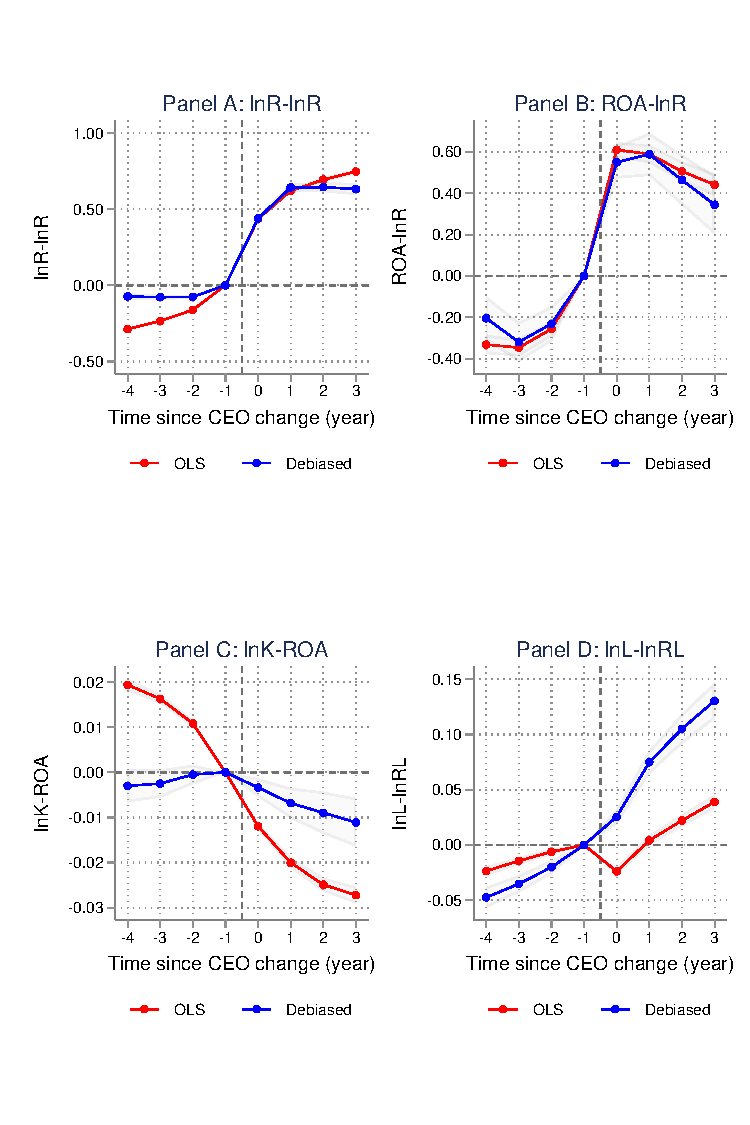
\includegraphics[width=10cm]{figure/outcomes.pdf}
\caption{Revenue Dynamics Around CEO Transitions in Hungarian Firms -- Selected Measures}
\label{fig:application}
\vspace{.3cm}
\begin{minipage}{0.9\textwidth}
\footnotesize
Notes: Event studies of various second moments around CEO transitions. All panels normalize to year $t=-1$ (one year before CEO arrival). Panel A shows the variance of revenue changes from baseline. Panel B plots the covariance of revenue change with the change in CEO fixed effect. Panel C displays the fraction of revenue variance explained by CEO fixed effects (R-squared). Panel D shows the variance of CEO fixed effects by firm age, decomposed into revenue shocks and CEO contributions. Panel E shows regression coefficients from projecting revenue on CEO effects, and Panel F shows the coefficients from regressing exporter status on CEO effect. Red lines show naive OLS estimates; blue lines show placebo-corrected debiased estimates. Shaded regions indicate 95\% confidence intervals. The placebo group consists of matched non-changing firms from the same birth cohort and sector, assigned pseudo CEO transitions at the same calendar year as treated firms. Event window spans $[-4, +3]$ years around CEO arrival.
\end{minipage}
\end{figure}


\begin{figure}[h]
    \centering
    
\includegraphics[width=13cm]{\figurepath/ceo-spell-distributions.pdf}
    
\includegraphics[width=13cm]{\figurepath/ceo-spell-distributions-weighted.pdf}
\begin{minipage}{10cm}
    \caption{CEO Tenure}
    \label{fig:tenure}
    \vspace{.3cm}
\footnotesize {Notes: Maximum tenure of the first CEO. Top panel: unweighted; Bottom panel: weighted by the number of years.} 
    \end{minipage}    
\end{figure}

\begin{figure}[h]
    \centering
    
\includegraphics[width=15cm]{\figurepath/tenure-snapshots.pdf}
\begin{minipage}{14.5 cm}
    \label{fig:tenure_year}
        \caption{CEO Tenure by Year}
\vspace{.3cm}
\footnotesize {Notes: Actual CEO tenure in various years.}
    \end{minipage}    
\end{figure}

\begin{figure}[htbp]
\centering
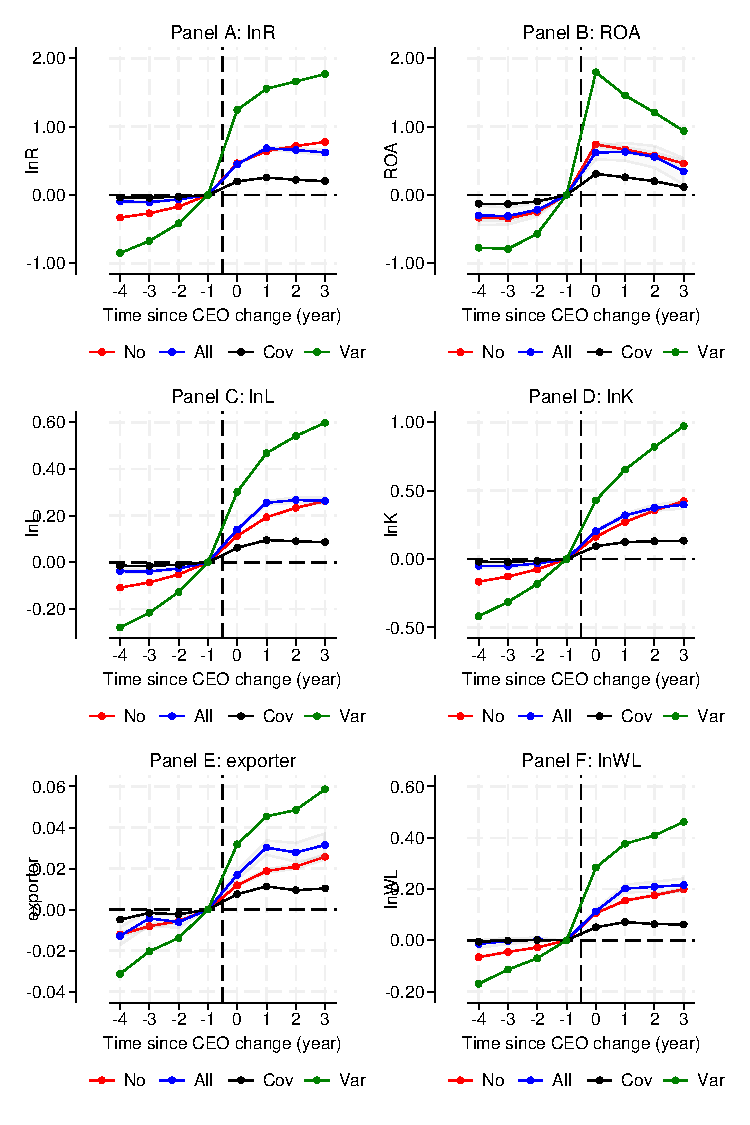
\includegraphics[width=10cm]{figure/outcomes_full_lnR.pdf}
\caption{Revenue Dynamics Around CEO Transitions in Hungarian Firms -- CEO Transition measured by Revenue}
\label{fig:application_lnR}
\vspace{.2cm}

\begin{minipage}{0.9\textwidth}
\footnotesize {Notes: Event-time dynamics of naive (red line) and placebo-controlled debiased (blue line) coefficients and 95\% confidence intervals. $\Delta z$ measured by $lnR$. $lnR$ = log revenue; Export = dummy variable = 1 if the firm exports in the given year; $lnL$ = log labor; $lnK$ = log tangible assets; ROA = return on assets; $lnRL$ = log labor productivity.}
\end{minipage}
\end{figure}

\begin{figure}[htbp]
\centering
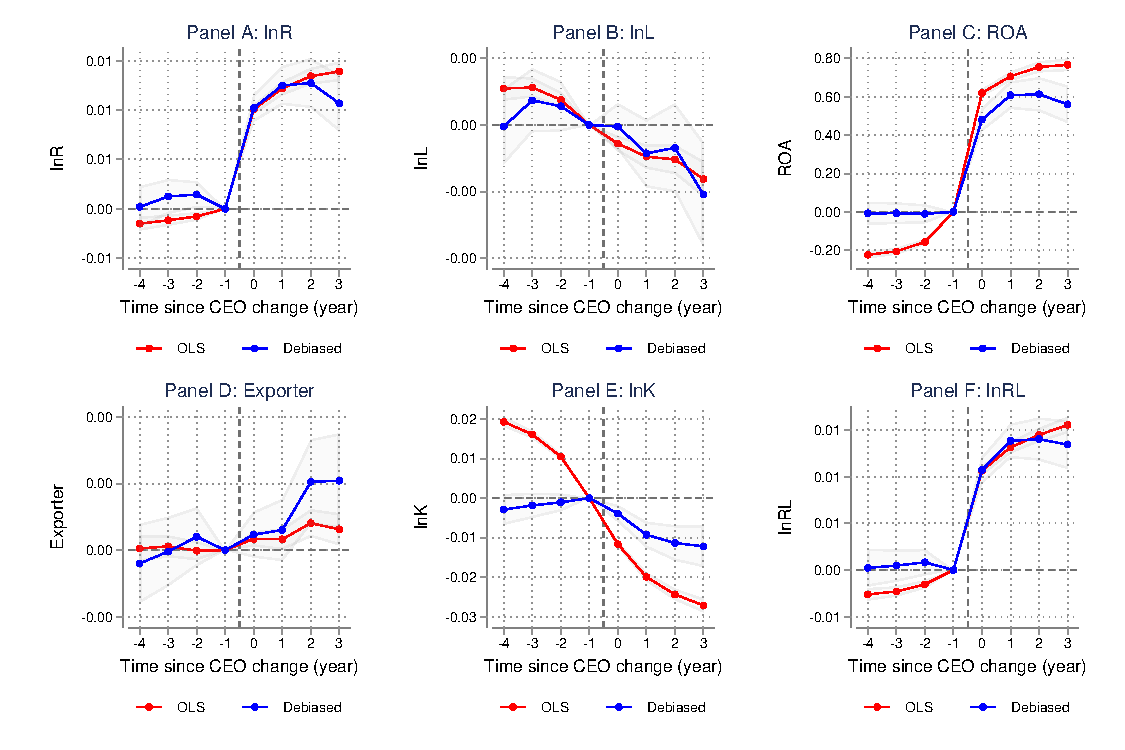
\includegraphics[width=10cm]{figure/outcomes_full_ROA.pdf}
\caption{Revenue Dynamics Around CEO Transitions in Hungarian Firms -- CEO Transition measured by Return on Assets}
\label{fig:application_ROA}
\vspace{.2cm}

\begin{minipage}{0.9\textwidth}
\footnotesize{Notes: Event-time dynamics of naive (red line) and placebo-controlled debiased (blue line) coefficients and 95\% confidence intervals. $\Delta z$ measured by ROA. $lnR$ = log revenue; Export = dummy variable = 1 if the firm exports in the given year; $lnL$ = log labor; $lnK$ = log tangible assets; ROA = return on assets; $lnRL$ = log labor productivity.}
\end{minipage}
\end{figure}

\begin{figure}[htbp]
\centering
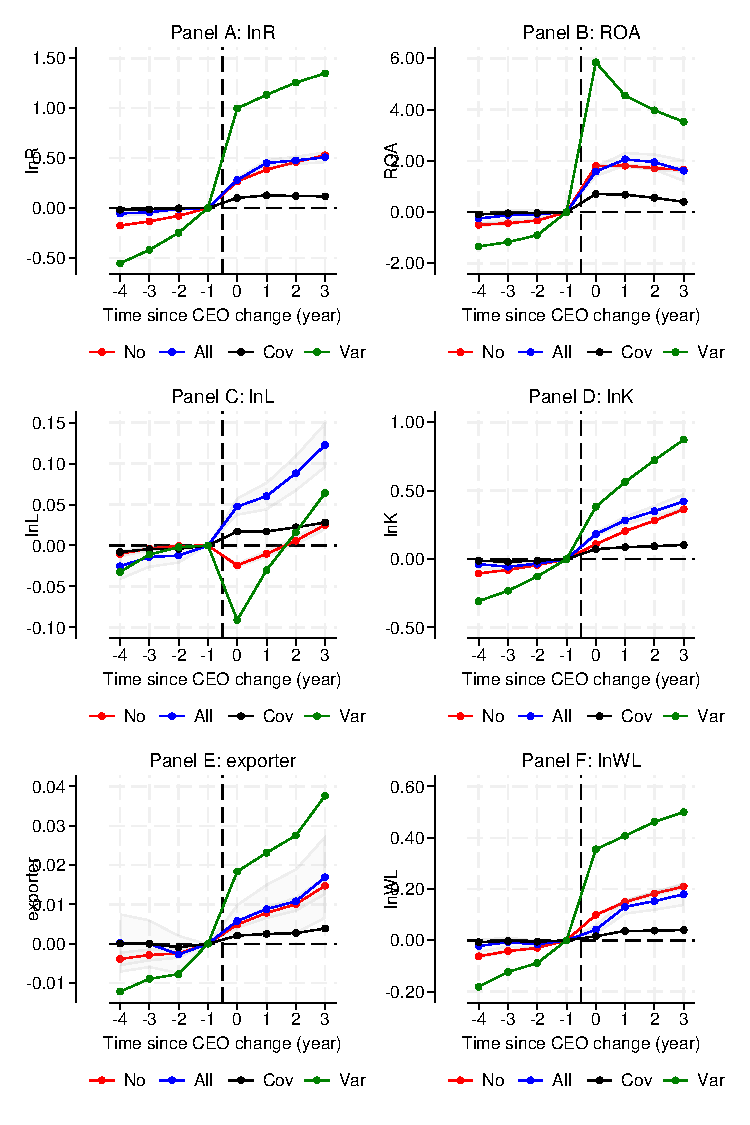
\includegraphics[width=10cm]{figure/outcomes_full_lnYL.pdf}
\caption{Revenue Dynamics Around CEO Transitions in Hungarian Firms -- CEO Transition measured by Labor Productivity}
\label{fig:application_lnYR}
\vspace{.2cm}

\begin{minipage}{0.9\textwidth}
\footnotesize {Notes: Event-time dynamics of naive (red line) and placebo-controlled debiased (blue line) coefficients and 95\% confidence intervals. $\Delta z$ measured by $lnRY$. $lnR$ = log revenue; Export = dummy variable = 1 if the firm exports in the given year; $lnL$ = log labor; $lnK$ = log tangible assets; ROA = return on assets; $lnRL$ = log labor productivity.} 
\end{minipage}
\end{figure}

\clearpage

\begin{table}[h]
    \centering
    \caption{Monte Carlo Parameters by Scenario}
    \vspace{.2cm}
    \label{tab:table_MC}
    & Baseline & Excess Variance & E. V. with Correction & Long Panel\\
\addlinespace$\hat Var(dz) (OLS) & $1.782^{}$ & $2.121^{}$ & $2.121^{}$ & $2.045^{}$ & \\
$\hat Var(dz)$ (debiased) & $1.003^{}$ & $1.343^{}$ & $1.343^{}$ & $1.019^{}$ & \\
\addlinespace$\hat Cov(dz, dy)$ (OLS) & $1.831^{}$ & $2.193^{}$ & $2.193^{}$ & $1.890^{}$ & \\
$\hat Cov(dz,dy)$ (debiased) & $0.996^{}$ & $1.365^{}$ & $1.191^{}$ & $1.013^{}$ & \\
\addlinespace $ R^2$ (Naive) & $0.808^{}$ & $0.779^{}$ & $0.779^{}$ & $0.643^{}$ & \\
$ R^2$ (debiased) & $0.608^{}$ & $0.622^{}$ & $0.520^{}$ & $0.578^{}$ & 
    \begin{minipage}{15.5cm}
    \vspace{.2cm}
    \footnotesize{Notes: Naive and placebo debiased coefficients and the values of the corresponding $R^2$ in Monte-Carlo simulations (50,000 treated firms and 50,000 control firms). Estimation of $\Delta z$ on lnR, when $\Delta z$ is measured by lnR. Treatment (placebo treatment) year drawn from a geometric distribution with a constant hazard of CEO change. Column 1 (baseline scenario): $\sigma(\Delta z) = 1$, $\sigma(\epsilon) = 0.71$, $\rho=0.9$, $T_1=T_2=4$; Column 2-3 (excess variance): $\sigma(\epsilon) = 1.2 \cdot 0.71$ in the treated group; Column 4 (long panel): firm spells are raised to $T_1=T_2=10$. $R^2$: the estimation based on all years (ATET); $R^2 \text{ at } t =3)$: the estimation is based on the difference between three years after relative to the year precedent to the treatment.}
    \end{minipage}
\end{table}
\vspace{.5cm}

\begin{table}
    \centering
    \caption{Characteristics of Firms With and Without a CEO Replacement}
    \vspace{.2cm}
    \label{tab:switch_desc}
    \begin{tabular}{lcccc}
    \begin{tabular}{lccccccc}
\hline\hline
 & lnR & Exporter & lnL & lnK & ROA & lnRL & N \\
\hline
Without CEO Switch & $10.0$ & $0.1$ & $1.4$ & $7.9$ & $2.5$ & $8.6$ & $220136$ \\
 & ($1.7$) & ($0.3$) & ($0.9$) & ($2.2$) & ($9.8$) & ($1.4$) &  \\
With CEO Switch & $10.2$ & $0.1$ & $1.5$ & $8.3$ & $2.2$ & $8.7$ & $231710$ \\
 & ($1.9$) & ($0.3$) & ($1.0$) & ($2.4$) & ($9.0$) & ($1.4$) &  \\
Growth & $-0.008$ & $-0.204$ & $-0.079$ & $-0.003$ & $-0.057$ & $0.004$ &  \\
 & ($0.185$) & ($0.760$) & ($0.657$) & ($0.284$) & ($374.204$) & ($0.192$) &  \\
Pre-trend & $0.004$ & $-0.154$ & $-0.007$ & $-0.003$ & $-0.080$ & $0.006$ &  \\
 & ($0.114$) & ($0.498$) & ($0.433$) & ($0.240$) & ($85.598$) & ($0.125$) &  \\
\hline\hline
\end{tabular}

    \end{tabular}
    \begin{minipage}{14.5cm}
    \vspace{.2cm}
    \footnotesize{Notes: this table shows the characteristics of firms with and without CEO replacement and the proportional change of firm characteristics around the CEO replacement.}
    \end{minipage}
\end{table}
\vspace{.5cm}


\begin{table}
    \centering
    \caption{Estimated Effect of CEO Change and $\text{R}^2$ -- Naive and Placebo-Controlled Debiased Methods }
    \vspace{.2cm}
    \label{tab:table_application}
    Estimate & lnR & ROA & lnL & lnK & exporter & lnWL\\
ATET (OLS) & $0.766^{}$ & $0.836^{}$ & $0.232^{}$ & $0.348^{}$ & $0.023^{}$ & $0.173^{}$\\
ATET (debiased) & $0.619^{}$ & $0.730^{}$ & $0.231^{}$ & $0.321^{}$ & $0.029^{}$ & $0.163^{}$\\
\addlinespace $ R^2$ (OLS) & $0.265^{}$ & $0.015^{}$ & $0.084^{}$ & $0.038^{}$ & $0.009^{}$ & $0.063^{}$\\
$ R^2$ (debiased) & $0.168^{}$ & $0.010^{}$ & $0.071^{}$ & $0.029^{}$ & $0.009^{}$ & $0.043^{}$\\
N & $2.6e+06^{}$ & $2.1e+06^{}$ & $2.6e+06^{}$ & $2.3e+06^{}$ & $2.6e+06^{}$ & $1.5e+06^{}$
    Estimate & lnR & exporter & lnL & lnK & ROA & lnYL\\
ATET (OLS) & $.^{}$ & $.^{}$ & $.^{}$ & $.^{}$ & $.^{}$ & $.^{}$\\
ATET (debiased) & $.^{}$ & $.^{}$ & $.^{}$ & $.^{}$ & $.^{}$ & $.^{}$\\
\addlinespace $ R^2$ (OLS) & $0.012^{}$ & $0.000^{}$ & $0.000^{}$ & $0.029^{}$ & $0.630^{}$ & $0.039^{}$\\
$ R^2$ (debiased) & $0.005^{}$ & $0.000^{}$ & $0.000^{}$ & $0.000^{}$ & $0.132^{}$ & $0.013^{}$\\
N & $2,326,279^{}$ & $2,495,873^{}$ & $2,495,873^{}$ & $2,305,547^{}$ & $2,495,873^{}$ & $1,811,955^{}$
    \begin{tabular}{l*{6}{c}}
\hline\hline
 Estimate & lnR & Exporter & lnL & lnK & ROA & lnRL \\
\hline
ATET (OLS) & $0.864^{***}$ & $0.021^{***}$ & $0.028^{***}$ & $0.292^{***}$ & $1.467^{**}$ & $0.837^{***}$ \\
ATET (debiased) & $0.879^{**}$ & $0.028^{***}$ & $0.105^{***}$ & $0.331^{***}$ & $1.416^{*}$ & $0.804^{**}$ \\
\addlinespace $ R^2$ (OLS) & $0.510^{}$ & $0.006^{}$ & $0.002^{}$ & $0.042^{}$ & $0.018^{}$ & $0.647^{}$ \\
$ R^2$ (debiased) & $0.254^{}$ & $0.005^{}$ & $0.013^{}$ & $0.026^{}$ & $0.008^{}$ & $0.289^{}$ \\
N & $2,551,515$ & $2,551,515$ & $2,551,515$ & $2,551,515$ & $2,551,515$ & $2,551,515$ \\
\hline\hline
\end{tabular}

    \begin{minipage}{16cm}
    \vspace{.2cm}
    \footnotesize{Notes: The table presents the naive and placebo-controlled debiased estimated coefficients and the corresponding $R^2$ of CEO replacement. The variable used for estimating $\Delta z$ is log revenue (top panel), return on assets (middle panel), log labor productivity (bottom panel). lnR = log revenue; Export = dummy variable = 1 if the firm exports in the given year; lnL = log labor; lnK = log tangible assets; ROA = return on assets; lnRL = log labor productivity.}
    \end{minipage}
\end{table}

\clearpage

%%%%%%%%%%%%%%%%%%%%%%%%%%%%%%%%%%%%%%%%%%%%%%
\section*{Appendix A: Derivation of Bias Terms}\label{sec: appA}
%%%%%%%%%%%%%%%%%%%%%%%%%%%%%%%%%%%%%%%%%%%%%%

\setcounter{equation}{0}
\renewcommand{\theequation}{A\arabic{equation}}

This appendix provides the formal matrix algebra derivation of the bias terms in second moments of estimated CEO effects.

\subsection{Matrix Notation Setup}

\paragraph{Model setup.} Let firm $i$ be observed for $T$ periods with outcome path $\mathbf y_i\in\mathbb R^T$ that decomposes into a (piecewise-constant) manager-effect path $\mathbf z_i$ and shocks $\mathbf e_i$. The model is
\begin{equation}
\mathbf y_i = \mathbf \alpha_i + \mathbf z_i + \mathbf e_i
\end{equation}
with 
\begin{equation}
\mathbb E[\mathbf z_i\mathbf z_i']= \mathbf \Lambda_i=
\begin{bmatrix}
  \lambda_{i11}\otimes \mathbf{11}' & \lambda_{i12}\otimes \mathbf{11}'\\
  \lambda_{i12}\otimes \mathbf{11}' & \lambda_{i22}\otimes \mathbf{11}'
\end{bmatrix},
\qquad \mathbb E[\mathbf z_i\mathbf e_i']=0,
\qquad \mathbb E[\mathbf e_i\mathbf e_i']=\sigma_1\mathbf\Sigma
\end{equation}
for changing firms, and 
\begin{equation}
\mathbb E[\mathbf z_i\mathbf z_i']= \mathbf \Lambda_i=
  \lambda_{i11}\otimes \mathbf{11}',
\qquad \mathbb E[\mathbf z_i\mathbf e_i']=0,
\qquad \mathbb E[\mathbf e_i\mathbf e_i']=\sigma_0\mathbf\Sigma
\end{equation}
for non-changing firms. The first equation is notation for the variance and covariance of manager fixed effects at firm $i$. The second equation states strict exogeneity (random mobility): every period's shock is mean independent of the entire CEO path. The third assumption allows for arbitrary autocorrelation in shocks over time but assumes that this autocorrelation is the same for changing and non-changing firms, up to a scalar multiplier $\sigma_1/\sigma_0$ (proportional autocovariance).

\paragraph{Projection Matrix and LSDV Estimator.} Define design matrix $\mathbf D$ and spell-length matrix $\mathbf T$. For $T_1=2$, $T_2=3$:
\[
  \mathbf D = \begin{bmatrix}
    1 & 0\\
    1 & 0\\
    0 & 1\\
    0 & 1\\
    0 & 1
  \end{bmatrix},
\]
and the diagonal matrix of spell lengths $\mathbf T$ as
$$
  \mathbf T = \operatorname{diag}(T_1,T_2)=\operatorname{diag}(2,3).
$$
The projection matrix that converts outcomes to within-spell means is
$$
  \mathbf P = \mathbf D\,\mathbf T^{-1}\,\mathbf D'.
$$
In the example,
\[
  \mathbf P = \begin{bmatrix}
    1/2 & 1/2 & 0 & 0 & 0\\
    1/2 & 1/2 & 0 & 0 & 0\\
    0 & 0 & 1/3 & 1/3 & 1/3\\
    0 & 0 & 1/3 & 1/3 & 1/3\\
    0 & 0 & 1/3 & 1/3 & 1/3
  \end{bmatrix}\quad\Rightarrow\quad
  \mathbf {Py}_i = 
  \mathbf\alpha_i +
  \begin{pmatrix}
  \frac12 \sum_{t=-2}^{-1} (z_{it} + e_{it}) \\
  \frac12 \sum_{t=-2}^{-1} (z_{it} + e_{it}) \\
  \frac13 \sum_{t=0}^{+2} (z_{it} + e_{it})\\
  \frac13 \sum_{t=0}^{+2} (z_{it} + e_{it})\\
  \frac13 \sum_{t=0}^{+2} (z_{it} + e_{it})
  \end{pmatrix}.
\]
Here $\mathbf P$ is idempotent, symmetric, and $\mathbf P\mathbf z_i = \mathbf z_i$.

The least-squares dummy variable (LSDV) estimator of the CEO effects is
\begin{equation}\label{eq:lsdv_appendix}
  \hat{\mathbf z}_i = \mathbf P\mathbf y_i - \hat{\mathbf \alpha}_i = \mathbf z_i + \mathbf P\mathbf e_i.
\end{equation}  
The estimated CEO effects are the true effects plus the within-spell mean of shocks. (For our method, it does not matter how firm fixed effects $\hat{\mathbf \alpha}_i$ are estimated, as we difference out firm means in all contrasts.)

\subsection{Population Moments and Bias Terms}

The relevant moments are
\begin{align}
  \mathbb E[\hat{\mathbf z_i}] &= \mathbf z_i,\\
  \mathbb E[\hat{\mathbf z_i}\hat{\mathbf z_i}'] &= 
\mathbb E[(\mathbf z_i + \mathbf P\mathbf e_i)(\mathbf z_i + \mathbf P\mathbf e_i)' ] =
    \mathbf \Lambda_i + \sigma\mathbf P\mathbf\Sigma\mathbf P,\\ 
  \mathbb E[\hat{\mathbf z_i}\mathbf e_i'] &= 
\mathbb E[(\mathbf z_i + \mathbf P\mathbf e_i)\mathbf e_i' ] = \sigma\mathbf P\mathbf\Sigma,\\
  \mathbb E[\hat{\mathbf z_i}\mathbf y_i'] &= 
\mathbb E[(\mathbf z_i + \mathbf P\mathbf e_i)(\mathbf z_i + \mathbf e_i)' ] = \mathbf \Lambda_i + \sigma\mathbf P\mathbf\Sigma.
\end{align}
These show variance inflation by $\sigma\mathbf P\mathbf\Sigma\mathbf P$ and contaminated covariances.

\subsection{Bias in Regression Slopes}

For any linear contrast with weights $\mathbf w\in\mathbb R^T$ and $\mathbf w'\mathbf 1=0$, define the estimated effect for the contrast by
$$
\Delta\hat z_i = \mathbf w'\hat{\mathbf z}_i = \mathbf w'\mathbf P\,\mathbf y_i = \Delta z_i + \eta_i,\qquad \eta_i:=\mathbf w'\mathbf P\,\mathbf e_i,
$$
and recall that $\Delta y_i = \Delta z_i + \varepsilon_i$ where $\varepsilon_i=\mathbf w'\mathbf e_i$. 

The naive regression slope is
\begin{equation}
\hat\beta = 
  \frac {\Cov(\Delta \hat z_i, \Delta y_i)}
        {\Var(\Delta \hat z_i)} =
  \frac {\mathbf w' \mathbb E[\hat{\mathbf z_i}\mathbf y_i ']\mathbf w}
        {\mathbf w' \mathbb E[\hat{\mathbf z_i}\hat{\mathbf z_i}']\mathbf w} =
  \frac {\mathbf w' [\mathbf \Lambda_i + \sigma \mathbf P\mathbf\Sigma]\mathbf w}
        {\mathbf w' [\mathbf \Lambda_i + \sigma \mathbf P\mathbf\Sigma\mathbf P]\mathbf w} =
  \frac {\lambda_i + \sigma \mathbf w' \mathbf P\mathbf\Sigma \mathbf w}
        {\lambda_i + \sigma \mathbf w' \mathbf P\mathbf\Sigma \mathbf P \mathbf w}. 
\end{equation}  

\textit{Covariance bias term.} $\Cov(\varepsilon_i,\eta_i)$ inflates the numerator when shocks are persistent and spells short.

\textit{Variance bias term.} $\Var(\eta_i)>0$ attenuates the denominator.

Both biases vanish as $T_1,T_2\to\infty$. 

\subsection{Sample Moments Across Heterogeneous Groups}

With $G$ groups of sizes $N_g$, sample moments are
\begin{align}
\widehat{\Cov}(\Delta y_i,\Delta \hat z_i) &= \sum_{g=1}^G \frac{N_g}{N} \widehat{\Cov}_g(\Delta y_i,\Delta \hat z_i)\\
\widehat{\Var}(\Delta \hat z_i) &= \sum_{g=1}^G \frac{N_g}{N} \widehat{\Var}_g(\Delta \hat z_i)
\end{align}

The expected values are
\begin{align}
\mathbb E\widehat{\Cov}(\Delta y_i,\Delta \hat z_i) &= \sum_{g=1}^G \frac{N_g}{N} \left[ 
\Bar\lambda_g
+ \sigma_g \mathbf w_g' \mathbf P_g\mathbf\Sigma \mathbf w_g\right] = 
\Bar\lambda +\sum_{g=1}^G \frac{N_g}{N} \sigma_g \mathbf w_g' \mathbf P_g\mathbf\Sigma \mathbf w_g\\
\mathbb E\widehat{\Var}(\Delta \hat z_i) &= \sum_{g=1}^G \frac{N_g}{N} \left[ 
\Bar\lambda_g
+ \sigma_g \mathbf w_g' \mathbf P_g\mathbf\Sigma \mathbf P_g \mathbf w_g\right] = 
\Bar\lambda +\sum_{g=1}^G \frac{N_g}{N} \sigma_g \mathbf w_g' \mathbf P_g\mathbf\Sigma \mathbf P_g \mathbf w_g
\end{align}

Here $\Bar\lambda$ is the average CEO effect variance. Bias terms depend on $\mathbf P_g$, $\mathbf w_g$, and $\sigma_g\mathbf\Sigma$, making direct estimation impractical with complex $\mathbf\Sigma$.

\clearpage

%%%%%%%%%%%%%%%%%%%%%%%%%%%%%%%%%%%%%
\section*{Appendix B: Additional Figures and Tables}
%%%%%%%%%%%%%%%%%%%%%%%%%%%%%%%%%%%%%

\renewcommand{\thefigure}{B\arabic{figure}} 
\renewcommand{\thetable}{B\arabic{table}}
\setcounter{figure}{0}
\setcounter{table}{0}

\begin{table}%[H]
    \centering
    \caption{Company-Year Characteristics}
    \vspace{.2cm}
    \label{tab:year_desc}
    \begin{tabular}{l*{3}{c}}
\hline\hline
Year & Frims & CEO Switches & Employment \\
\hline
1995  & 76866 & 3921 & 13 \\
2000  & 133686 & 10043 & 10 \\
2005  & 145956 & 8772 & 9 \\
2010  & 138815 & 8684 & 9 \\
2015  & 158242 & 10733 & 9 \\
2020  & 174683 & 10714 & 9 \\
Total  & 4107611 & 262973 & 10 \\
\hline\hline
\end{tabular}

    \begin{minipage}{9cm}
    \vspace{.2cm}
    \footnotesize{Notes: the table presents the number of firms, number of CEO replacements, and average employment of firms in each year of the data.}
    \end{minipage}
\end{table}
\vspace{.5cm}


\begin{table}[H]
    \centering
    \caption{Industrial Distribution of Firms}
    \vspace{.2cm}
    \label{tab:industry_desc}
    \begin{tabular}{l*{2}{c}}
\hline\hline
Industry & N & \% \\
\hline
Agriculture & $141867$ & $3.5$ \\
Industry & $578437$ & $14.1$ \\
Construction & $447245$ & $10.9$ \\
Trade & $1122181$ & $27.3$ \\
Business Services & $662333$ & $16.1$ \\
Other Services & $1155548$ & $28.1$ \\
\hline\hline
\end{tabular}

    \begin{minipage}{13cm}
    \vspace{.2cm}
    \footnotesize{Notes: Distribution of firms by sector.}
    \end{minipage}
\end{table}
\vspace{.5cm}


\begin{table}[H]
    \centering
    \caption{CEO Tenure}
    \vspace{.2cm}
    \label{tab:tenure_desc}
    \begin{tabular}{lcccc}
    \begin{tabular}{l*{3}{c}}
\hline\hline
Statistic & P25 & P50 & P75 \\
\hline
Firm max age & $.$ & $.$ & $.$ \\
1st CEO tenure & $2.00$ & $5.00$ & $10.00$ \\
2nd CEO tenure & $2.00$ & $4.00$ & $8.00$ \\
3rd CEO tenure & $2.00$ & $4.00$ & $7.00$ \\
4th or higher CEO tenure & $2.00$ & $3.00$ & $6.00$ \\
% of firms with 2 CEOs & $0.28$ & $.$ & $.$ \\
% of firms with CEO switches & $0.48$ & $.$ & $.$ \\
Nr. of Firms & $537998.00$ & $.$ & $.$ \\
\hline\hline
\end{tabular}

    \end{tabular}
    \begin{minipage}{10cm}
    \vspace{.2cm}
    \footnotesize{Notes: distribution of the length of tenure of CEOs. Tenure measured in years.}
    \end{minipage}
\end{table}
\vspace{.5cm}

\end{document}
